\clearpage
\textbf{Supplementary Note 7. The yield-model lineage and the gamma–Poisson family (Sections 1 and 3.1 of the main text).}

\textit{The die-yield lineage.} The earliest die-yield model assumes defects that are Poisson-distributed over the wafer with density $D_{0}$, so that a die of area $A$ is defect-free with probability $\exp(-AD_{0})$. Observed yields exceeded this prediction for large dies, and the explanation---defect density varies across wafers and across regions of a wafer---led Murphy (1964) to average the Poisson yield over a triangular distribution of $D_{0}$ and Seeds (1967) and Price (1970) over an exponential distribution. Stapper (1973) and Stapper et al.\ (1983) generalised the mixture to a gamma distribution, which yields the negative-binomial formula (Y2) below with a cluster parameter $\alpha$. The negative-binomial model became standard because $\alpha$ could be estimated from wafer maps and because it nests the earlier forms (Cunningham, 1990; Stapper, 1989). Defect density itself follows a learning curve that is well approximated by a log-linear decline in cumulative volume (Wright, 1936), and yield engineers use the fitted $(D_{0},\alpha)$ to set scrap and disposition limits and to select among model variants with information criteria. Fig.~S1(a) summarises this lineage, each model drawn as the distribution of defect density over which it averages the Poisson yield.

\textit{The source model.} For a die of area $A$ on a wafer with defect density $D_{0}$ and cluster parameter $\alpha$, the source model of Section 3.1 of the main text can be stated in four expressions,
\begin{align}
Y_{\mathrm{Poisson}} &= \exp(-AD_{0}), \tag{Y1}\\
Y_{\mathrm{NB}} &= \Big(1 + \frac{AD_{0}}{\alpha}\Big)^{-\alpha}, \tag{Y2}\\
\log D_{0}(v) &= a_{0} - b_{0}\log v, \tag{Y3}\\
\text{scrap rate} &= 1 - Y_{\mathrm{NB}}\ \text{(die level)}, \tag{Y4}
\end{align}
where $v$ is cumulative volume and (Y3) is the learning curve. In the source, $(D_{0},\alpha)$ are estimated from inspection data, (Y3) is fitted by least squares and scrap limits are set as control limits on yield; Sections 3.2--4.4 of the main text replace each of these steps, and Fig.~S4 draws the three-layer correspondence---detection, model, alarm---between the two readings.

\noindent\begin{minipage}{\linewidth}\centering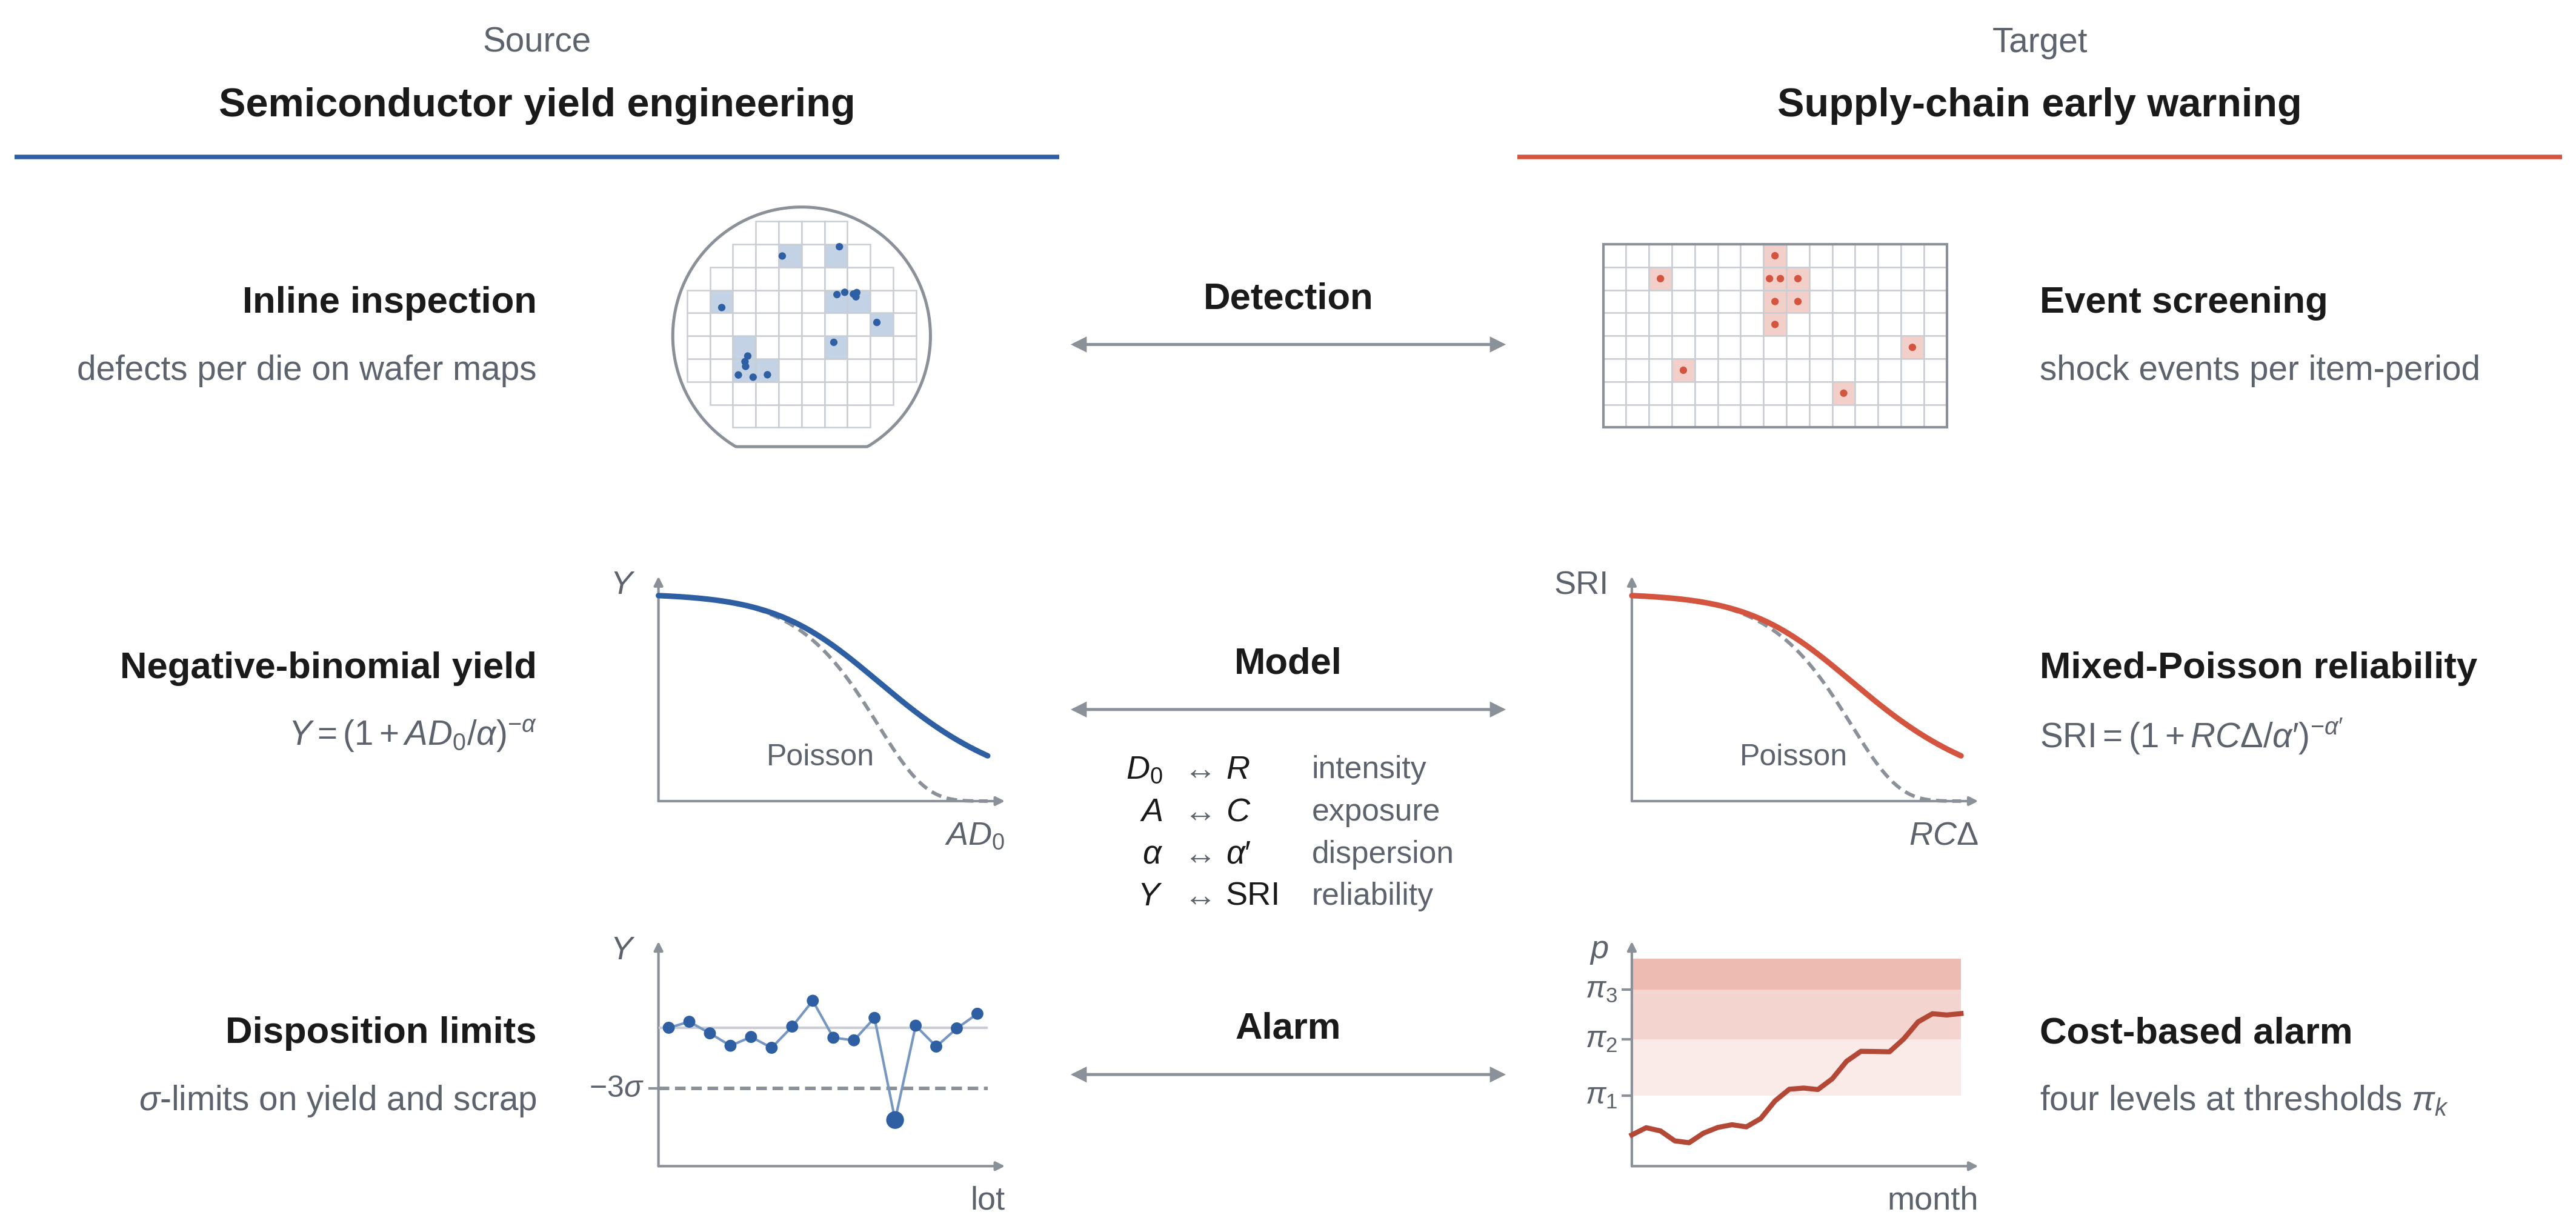
\includegraphics[width=\linewidth]{figs/FigS4_correspondence.png}
\captionof{figure}{Fig. S4. Three-layer correspondence between semiconductor yield engineering (source) and supply-chain early warning (target): inline inspection and event screening (detection), negative-binomial yield and mixed-Poisson reliability (model), disposition limits and the cost-based alarm (alarm).}\label{fig:S4}\end{minipage}
\vspace{14pt}

\textit{The gamma–Poisson family across domains.} The negative-binomial yield model is one instance of a much older idea: a Poisson process whose intensity is itself gamma-distributed, so that heterogeneity of the intensity produces over-dispersion and the probability of zero events is the Laplace transform of the intensity distribution evaluated at the exposure. Greenwood and Yule's accident proneness (1920), the CreditRisk+ model of portfolio default counts (Credit Suisse Financial Products, 1997), the dispersion parameter of superspreading (Lloyd-Smith et al., 2005), gamma frailty in survival and reliability analysis (Vaupel et al., 1979; Hougaard, 2000) and the general theory of mixed Poisson processes (Grandell, 1997) all rest on this construction; software-reliability growth models (Goel and Okumoto, 1979) play the role of the learning curve, and count-regression practice made the negative binomial the default for over-dispersed counts (Lawless, 1987; Cameron and Trivedi, 2013). Fig.~S1(b) summarises this genealogy around the zero-probability identity at its centre, with the supply-shock case of the main text below. Table S17 gives the variable correspondence between the source (die yield) and target (supply reliability) readings that Fig.~S4 draws (Section 1 of the main text).

\noindent\begin{minipage}{\linewidth}\centering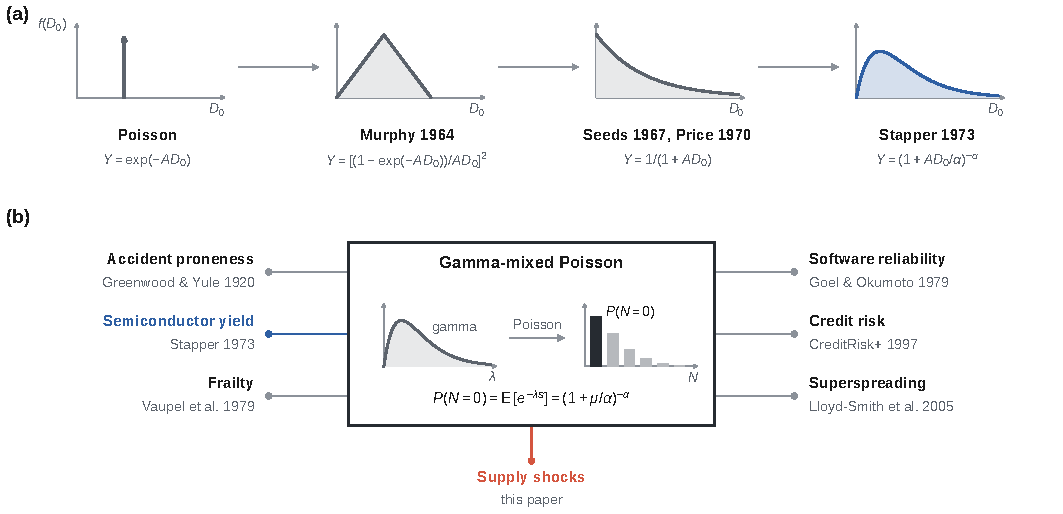
\includegraphics[width=\linewidth]{figs/FigS1_lineages.pdf}
\captionof{figure}{Fig. S1. (a) Die-yield model lineage from the Poisson formula to the negative binomial; (b) the gamma–Poisson family across domains.}\label{fig:S1}\end{minipage}
\vspace{14pt}

\noindent\begin{minipage}{\linewidth}
\captionof{table}{Table S17. Variable correspondence between the source (die yield) and target (supply reliability) models (Fig.~S4; Section 1 of the main text).}\label{tab:S17}
\centering\footnotesize
\begin{tabular}{p{3.1cm}lp{5.9cm}ll}
\toprule
Source (yield) & Symbol & Target (supply) & Symbol & Role \\ \midrule
defect density (defects per unit area) & $D_{0}$ & risk intensity (expected shocks per period for a reference item) & $R_{it}$ & intensity \\
die area & $A$ & exposure coefficient (dimensionless multiplier of expected shocks) & $C_{i}$ & exposure \\
cluster parameter & $\alpha$ & dispersion parameter (within-period clustering of intensity) & $\alpha'_{g}$ & dispersion \\
defects per die & – & shock events per item-period & $N_{it}$ & count \\
expected defects per die & $AD_{0}$ & expected shocks per item-period & $\mu_{it} = R_{it}C_{i}\Delta$ & mean \\
die yield & $Y$ & supply reliability index, $P(N_{it} = 0)$ & $\mathrm{SRI}_{it}$ & reliability \\
scrap rate & – & supply disruption rate (Supplementary Note 8) & $\mathrm{SDR}_{it}$ & loss \\
learning curve in cumulative volume & (Y3) & group-level dynamic log-intensity & $m_{t}^{g},\delta_{t}^{g}$ & dynamics \\
\bottomrule
\end{tabular}
\end{minipage}
\vspace{14pt}

\textbf{Supplementary Note 8. Severity and the supply disruption rate (Section 4.4 of the main text).}

The SRI answers ``will there be a shock?''; the disruption rate answers ``how much supply is lost?'' Because a period without shocks has zero loss, the loss variable has a point mass at zero and the natural model is a hurdle,
\begin{align}\mathrm{SDR}_{it} &= \mathbf{1}\{N_{it}\ge 1\}\,S_{it}, \tag{S8.1}\\ S_{it}\mid N_{it}\ge 1 &\sim \mathrm{Beta}\big(\phi\,m_{it},\ \phi\,(1-m_{it})\big), \tag{S8.2}\\ \mathrm{logit}\,m_{it} &= \gamma_{0} + \gamma_{1}\log\mu_{it} + \boldsymbol{\gamma}_{2}^{\top}\mathbf{x}_{i,t-1}\ (+\,\gamma_{3}\log N_{it}), \tag{S8.3}\\ E[\mathrm{SDR}_{it}] &= (1-\mathrm{SRI}_{it})\,m_{it},\qquad E[\mathrm{Loss}_{it}] = \mu_{it}\,E[S_{it}], \tag{S8.4}\end{align}
where (S8.2)–(S8.3) is a beta regression (Ferrari and Cribari-Neto, 2004) for the loss fraction given a shock, with precision $\phi$, and the second equality in (S8.4) assumes losses add across shocks; the optional term in parentheses in (S8.3) lets the loss fraction depend on the number of shocks realised in the period. The two outputs of the framework---probability of disruption and loss given disruption---thus come from (4) of the main text and (S8.2) respectively. If complete stoppage ($S = 1$) can occur, a one-inflated beta or the compression of Smithson and Verkuilen (2006) is used (Ospina and Ferrari, 2010). For heavy-tailed severities the beta body is complemented by a generalised-Pareto tail fitted to exceedances of the observed loss fraction over its 90th percentile by the peaks-over-threshold method (Pickands, 1975; Coles, 2001), once at least ten exceedances are available (Section 4.4 of the main text). The priors are $\phi \sim \mathrm{Gamma}(2, 0.1)$ and $\gamma \sim N(0,1)$; the severity submodel is fitted at every monitoring origin, and its recovery of the design and the coverage of its loss-fraction intervals before and after conformalisation are reported in Table S15.

\textbf{Supplementary Note 9. Industry instances of the intensity–exposure–dispersion structure (Section 6.2 of the main text).}

The intensity–exposure–dispersion structure of Proposition 1 is not specific to critical materials. Table S18 instantiates $(\lambda, s, \alpha) \equiv (R, C, \alpha')$ for five industries at two levels: the process level, where the source model already operates in a form adapted to each industry, and the supply level, where the framework applies to the industry's own critical inputs. Fig.~S2 shows the dual application. The detection layer differs in every row; the model and alarm layers do not.

\begin{landscape}
\noindent\begin{minipage}{\linewidth}
\captionof{table}{Table S18. Industry instances of the intensity–exposure–dispersion structure.}\label{tab:S18}
\centering\scriptsize
\begin{tabular}{p{2.4cm}p{4.2cm}p{3.0cm}p{3.0cm}p{3.4cm}p{3.2cm}p{3.2cm}}
\toprule
Industry & Detection source & Intensity $\lambda$ ($= R$) & Exposure $s$ ($= C$) & Clustering $\alpha$ ($= \alpha'$) & Process-level output & Supply-level instance \\ \midrule
lithium-ion batteries & electrode vision, X-ray CT, field battery-management data & electrode defect density & cell area / capacity & coating-roll and lot correlation & cell yield / lot scrap & precursors, separators \\
displays & pixel inspection images (mura) & pixel defect density & panel area & spatial mura clustering & panel yield / substrate breakage & emitter materials \\
biopharmaceuticals & bioreactor sensors, GMP deviation records & contamination / deviation intensity & batch scale and value & raw-material lot and facility correlation & batch purity / batch rejection & media, chromatography resins \\
AI data centres & GPU telemetry (ECC errors, thermal) & node failure intensity & cluster and job size & rack- and power-level common cause & job completion / node uptime & high-bandwidth memory, accelerators \\
space systems & component qualification tests, on-orbit telemetry & component failure intensity & mission duration, orbital environment & common-cause failures & mission success / vehicle loss & space-grade components \\
\bottomrule
\end{tabular}
\end{minipage}
\vspace{14pt}

\noindent\begin{minipage}{\linewidth}\centering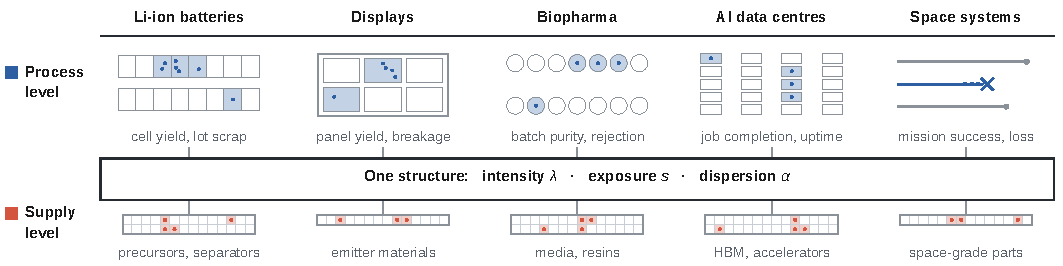
\includegraphics[width=0.9\linewidth]{figs/FigS2_industry_map.pdf}
\captionof{figure}{Fig. S2. Industry instance map: the intensity–exposure–dispersion structure at process level and at supply level.}\label{fig:S2}\end{minipage}
\end{landscape}
\textbf{Supplementary Note 10. Expected cost of the alarm policies (Section 5.6 of the main text).}

\textit{Inputs.} All quantities come from the archived replication-level results of Study B (\path{results/B/<cell>__all.jsonl}, 65 replications in 12 cells) and the follow-up baselines (\path{A3_farrington_replications.csv}, \path{B1_nbcharts_replications_group.csv}): for method $m$ at level $k$ in replication $j$, the one-month detection rate $\mathrm{DR}_{mkj}$ (\texttt{dr\_h1}), the share of decision item-months with the level in force (\texttt{alarm\_share}; alarm months per item-year $\mathrm{AM} = 12\times$ share), the number of alarm onsets (\texttt{n\_onsets}) and the false onsets per item-year over the whole window (\texttt{fa\_per\_itemyear}) and in the stable windows (\texttt{fa\_per\_itemyear\_stable}, the Table 6 quantity). The number of realised shock item-months in the detection window ($\tau = 37,\dots,118$) is counted exactly by regenerating each simulated panel from its archived seed (\path{dgp.simulate}, \path{dgp.seed_of('B', cell, rep)}); the regeneration reproduces the archived base rates and the EWMA/CUSUM metrics of all 65 replications to four decimals (\path{code/tools/validate_regen.py}).

\textit{Model A (main text).} $\mathrm{EC}_{mkj}(r) = \mathrm{AM}_{mkj} + r\,(1-\mathrm{DR}_{mkj})\,E_{j}$, with $E_{j}$ the shock item-months per item-year; never acting costs $rE_{j}$, always acting 12. For methods with several operating points the reported value at each $r$ is the cheapest of their levels (the lower envelope of the level-wise mean-cost lines); charts and the Farrington-type threshold have one line. Model A charges every alarm month, including those preceding a detected shock. The alternative that charges only alarm months not followed by a shock cannot be computed from the archived outputs, which hold alarm months and detection rates but not the alarm paths.

\textit{Model B (the classification framing of eq.\ (19) and of Table 6).} $\mathrm{EC}^{B}_{mkj}(r) = \mathrm{FA}_{mkj} + r\,(1-\mathrm{DR}_{mkj})\,E_{j}$ with $\mathrm{FA}$ the false onsets per item-year over the whole window. An onset is counted once however long the alarm stays on, so the always-on policy has almost no onsets and a cost of zero, and every probability-based method is cheapest at its lowest threshold for every $r$ (Table S22). Model B is reported to tie the cost analysis to the false-alarm definition of Table 6; the conclusions of the main text rest on Model A.

\textit{Statistics.} Means over the 65 replications (the reference cell has 10) with Monte Carlo standard errors; paired differences M2 $-$ $m$ at each method's cheapest level with two-sided sign tests; savings $1 - \mathrm{EC}_{\mathrm{M2}}/\mathrm{EC}_{m}$ on the means; break-even ratios $r^{*}$ where the envelope curves cross (log grid of 600 points on $[1, 100]$); the value of monitoring $1 - \mathrm{EC}_{\mathrm{M2}} / \min(rE, 12)$. Scripts: \path{code/tools/extract_alarm_share.py}, \path{code/tools/cost_curves.py}; outputs under \path{results/analysis/cost/}.

\noindent\begin{minipage}{\linewidth}
\captionof{table}{Table S19.1. Expected cost per item-year (Model A; units of one alarm-month), all twelve cells (n = 65): mean over replications (Monte Carlo standard error) at the method's cheapest level [L$k$] for each avoidable loss per shock $r$. Never act = $rE$; always act = 12.}\label{tab:S19.1}
\centering\scriptsize
\begin{tabular}{lrrrrr}
\toprule
Method & $r = 2$ & $r = 5$ & $r = 10$ & $r = 20$ & $r = 50$ \\ \midrule
M2 (proposed) & 5.18 (0.34) [L3] & 8.03 (0.35) [L3] & 10.47 (0.22) [L2] & 12.02 (0.06) [L1] & 12.91 (0.08) [L1] \\
NB complete pooling & 5.26 (0.34) [L3] & 8.08 (0.35) [L3] & 10.52 (0.22) [L2] & 12.02 (0.06) [L1] & 12.88 (0.08) [L1] \\
NB no pooling & 5.26 (0.33) [L3] & 8.10 (0.35) [L3] & 10.48 (0.22) [L2] & 11.94 (0.08) [L1] & 13.17 (0.08) [L1] \\
Poisson M0 & 5.42 (0.34) [L3] & 8.15 (0.36) [L3] & 10.53 (0.22) [L2] & 12.01 (0.06) [L1] & 12.91 (0.08) [L1] \\
XGBoost & 4.91 (0.32) [L3] & 8.76 (0.42) [L3] & 10.79 (0.21) [L2] & 12.19 (0.04) [L1] & 12.95 (0.08) [L1] \\
LSTM & 5.05 (0.33) [L3] & 8.78 (0.42) [L3] & 10.95 (0.20) [L2] & 12.18 (0.05) [L1] & 13.07 (0.08) [L1] \\
TFT & 4.98 (0.33) [L3] & 8.97 (0.44) [L3] & 11.07 (0.22) [L2] & 12.19 (0.05) [L1] & 13.18 (0.09) [L1] \\
Sigma-rule (plug-in SRI) & 5.05 (0.25) [L3] & 10.06 (0.47) [L1] & 16.96 (0.90) [L1] & 30.77 (1.78) [L1] & 72.21 (4.42) [L1] \\
EWMA & 5.56 (0.26) & 9.85 (0.46) & 16.99 (0.82) & 31.27 (1.55) & 74.13 (3.74) \\
CUSUM & 5.18 (0.29) & 9.47 (0.47) & 16.62 (0.79) & 30.92 (1.44) & 73.83 (3.41) \\
CUSUM, negative-binomial design & 5.08 (0.29) & 9.73 (0.50) & 17.47 (0.88) & 32.95 (1.65) & 79.41 (3.99) \\
Farrington-type threshold & 4.64 (0.28) & 10.96 (0.69) & 21.49 (1.38) & 42.56 (2.74) & 105.76 (6.84) \\
Never act & 4.44 (0.29) & 11.10 (0.73) & 22.21 (1.46) & 44.42 (2.92) & 111.04 (7.30) \\
Always act & 12.00 (0.00) & 12.00 (0.00) & 12.00 (0.00) & 12.00 (0.00) & 12.00 (0.00) \\
\bottomrule
\end{tabular}
\end{minipage}
\vspace{14pt}

\noindent\begin{minipage}{\linewidth}
\captionof{table}{Table S19.2. Expected cost per item-year (Model A; units of one alarm-month), cells with $\bar{\mu}$ = 0.05 (n = 30): mean over replications (Monte Carlo standard error) at the method's cheapest level [L$k$] for each avoidable loss per shock $r$. Never act = $rE$; always act = 12.}\label{tab:S19.2}
\centering\scriptsize
\begin{tabular}{lrrrrr}
\toprule
Method & $r = 2$ & $r = 5$ & $r = 10$ & $r = 20$ & $r = 50$ \\ \midrule
M2 (proposed) & 2.59 (0.18) [L3] & 5.31 (0.26) [L3] & 8.84 (0.24) [L2] & 11.58 (0.07) [L1] & 12.54 (0.10) [L1] \\
NB complete pooling & 2.63 (0.18) [L3] & 5.34 (0.26) [L3] & 8.94 (0.24) [L2] & 11.57 (0.07) [L1] & 12.47 (0.09) [L1] \\
NB no pooling & 2.68 (0.18) [L3] & 5.34 (0.26) [L3] & 8.92 (0.25) [L2] & 11.41 (0.10) [L1] & 13.04 (0.15) [L1] \\
Poisson M0 & 2.73 (0.20) [L3] & 5.36 (0.27) [L3] & 8.92 (0.24) [L2] & 11.58 (0.08) [L1] & 12.54 (0.12) [L1] \\
XGBoost & 2.32 (0.13) [L3] & 5.59 (0.30) [L3] & 9.29 (0.27) [L2] & 11.94 (0.06) [L1] & 12.64 (0.11) [L1] \\
LSTM & 2.39 (0.14) [L3] & 5.59 (0.30) [L3] & 9.55 (0.24) [L2] & 11.90 (0.06) [L1] & 12.82 (0.13) [L1] \\
TFT & 2.36 (0.13) [L3] & 5.62 (0.30) [L3] & 9.55 (0.29) [L2] & 11.91 (0.07) [L1] & 13.04 (0.17) [L1] \\
Sigma-rule (plug-in SRI) & 3.24 (0.14) [L3] & 6.00 (0.28) [L3] & 10.12 (0.40) [L1] & 17.17 (0.73) [L1] & 38.31 (1.74) [L1] \\
EWMA & 3.73 (0.21) & 6.21 (0.29) & 10.33 (0.44) & 18.57 (0.73) & 43.30 (1.64) \\
CUSUM & 3.01 (0.20) & 5.75 (0.29) & 10.30 (0.45) & 19.40 (0.77) & 46.72 (1.76) \\
CUSUM, negative-binomial design & 2.98 (0.20) & 5.74 (0.30) & 10.34 (0.46) & 19.54 (0.79) & 47.15 (1.81) \\
Farrington-type threshold & 2.53 (0.13) & 5.79 (0.31) & 11.23 (0.61) & 22.11 (1.20) & 54.74 (3.00) \\
Never act & 2.27 (0.13) & 5.67 (0.32) & 11.33 (0.63) & 22.67 (1.27) & 56.67 (3.17) \\
Always act & 12.00 (0.00) & 12.00 (0.00) & 12.00 (0.00) & 12.00 (0.00) & 12.00 (0.00) \\
\bottomrule
\end{tabular}
\end{minipage}
\vspace{14pt}

\noindent\begin{minipage}{\linewidth}
\captionof{table}{Table S19.3. Expected cost per item-year (Model A; units of one alarm-month), cells with $\bar{\mu}$ = 0.2 (n = 35): mean over replications (Monte Carlo standard error) at the method's cheapest level [L$k$] for each avoidable loss per shock $r$. Never act = $rE$; always act = 12.}\label{tab:S19.3}
\centering\scriptsize
\begin{tabular}{lrrrrr}
\toprule
Method & $r = 2$ & $r = 5$ & $r = 10$ & $r = 20$ & $r = 50$ \\ \midrule
M2 (proposed) & 7.41 (0.24) [L3] & 10.37 (0.15) [L3] & 11.86 (0.06) [L2] & 12.39 (0.03) [L1] & 13.23 (0.08) [L1] \\
NB complete pooling & 7.51 (0.24) [L3] & 10.43 (0.15) [L3] & 11.87 (0.05) [L2] & 12.40 (0.03) [L1] & 13.24 (0.08) [L1] \\
NB no pooling & 7.46 (0.22) [L3] & 10.47 (0.16) [L3] & 11.82 (0.07) [L2] & 12.38 (0.04) [L1] & 13.29 (0.09) [L1] \\
Poisson M0 & 7.71 (0.21) [L3] & 10.53 (0.18) [L3] & 11.92 (0.05) [L2] & 12.39 (0.03) [L1] & 13.22 (0.08) [L1] \\
XGBoost & 7.14 (0.20) [L3] & 11.47 (0.26) [L3] & 12.08 (0.04) [L2] & 12.40 (0.03) [L1] & 13.23 (0.08) [L1] \\
LSTM & 7.33 (0.18) [L3] & 11.52 (0.25) [L3] & 12.13 (0.02) [L1] & 12.42 (0.03) [L1] & 13.28 (0.09) [L1] \\
TFT & 7.23 (0.19) [L3] & 11.66 (0.05) [L2] & 12.13 (0.02) [L1] & 12.42 (0.04) [L1] & 13.30 (0.09) [L1] \\
Sigma-rule (plug-in SRI) & 6.59 (0.23) [L3] & 13.02 (0.40) [L1] & 22.83 (0.74) [L1] & 42.44 (1.43) [L1] & 101.26 (3.50) [L1] \\
EWMA & 7.13 (0.23) & 12.97 (0.27) & 22.70 (0.38) & 42.16 (0.66) & 100.55 (1.59) \\
CUSUM & 7.03 (0.23) & 12.66 (0.24) & 22.04 (0.38) & 40.80 (0.76) & 97.07 (2.01) \\
CUSUM, negative-binomial design & 6.88 (0.25) & 13.14 (0.29) & 23.58 (0.44) & 44.45 (0.83) & 107.06 (2.12) \\
Farrington-type threshold & 6.45 (0.25) & 15.39 (0.60) & 30.29 (1.19) & 60.09 (2.38) & 149.48 (5.94) \\
Never act & 6.31 (0.25) & 15.77 (0.64) & 31.53 (1.27) & 63.06 (2.55) & 157.65 (6.37) \\
Always act & 12.00 (0.00) & 12.00 (0.00) & 12.00 (0.00) & 12.00 (0.00) & 12.00 (0.00) \\
\bottomrule
\end{tabular}
\end{minipage}
\vspace{14pt}

\begin{landscape}
\noindent\begin{minipage}{\linewidth}
\captionof{table}{Table S20. Saving of M2 relative to each policy, all twelve cells (Model A): $1 - \mathrm{EC}_{\mathrm{M2}}/\mathrm{EC}_{m}$ on the means (share of the 65 replications in which M2 is cheaper; two-sided sign-test p-value, ties excluded), each method at its cheapest level. The last row takes the cheaper of never acting and always acting in each replication, so its benchmark is the mean of $\min(rE_j, 12)$. This benchmark never costs more than $\min(rE, 12)$ at the mean shock frequency of the subset, which Table S21.1 and the main text use for the value of monitoring. The savings in the last row are therefore never larger than the value of monitoring.}\label{tab:S20}
\centering\scriptsize
\begin{tabular}{llllll}
\toprule
Compared with & $r = 2$ & $r = 5$ & $r = 10$ & $r = 20$ & $r = 50$ \\ \midrule
NB complete pooling & +1.4\% (85\%; $<$0.001) & +0.6\% (63\%; 0.05) & +0.5\% (65\%; 0.02) & -0.0\% (52\%; 0.88) & -0.2\% (48\%; 0.88) \\
NB no pooling & +1.4\% (77\%; $<$0.001) & +0.8\% (68\%; 0.01) & +0.2\% (46\%; 0.62) & -0.7\% (32\%; 0.01) & +2.0\% (65\%; 0.03) \\
Poisson M0 & +4.3\% (82\%; $<$0.001) & +1.4\% (69\%; 0.00) & +0.7\% (66\%; 0.02) & -0.0\% (44\%; 0.47) & -0.1\% (46\%; 0.67) \\
XGBoost & -5.5\% (15\%; $<$0.001) & +8.3\% (91\%; $<$0.001) & +3.0\% (88\%; $<$0.001) & +1.4\% (88\%; $<$0.001) & +0.3\% (60\%; 0.19) \\
LSTM & -2.7\% (26\%; $<$0.001) & +8.6\% (95\%; $<$0.001) & +4.4\% (95\%; $<$0.001) & +1.3\% (90\%; $<$0.001) & +1.2\% (71\%; 0.01) \\
TFT & -4.0\% (20\%; $<$0.001) & +10.5\% (97\%; $<$0.001) & +5.5\% (97\%; $<$0.001) & +1.4\% (80\%; $<$0.001) & +2.0\% (67\%; 0.02) \\
Sigma-rule (plug-in SRI) & -2.7\% (43\%; 0.32) & +20.1\% (100\%; $<$0.001) & +38.3\% (97\%; $<$0.001) & +60.9\% (98\%; $<$0.001) & +82.1\% (100\%; $<$0.001) \\
EWMA & +6.8\% (54\%; 0.62) & +18.4\% (100\%; $<$0.001) & +38.4\% (94\%; $<$0.001) & +61.6\% (100\%; $<$0.001) & +82.6\% (100\%; $<$0.001) \\
CUSUM & -0.1\% (46\%; 0.62) & +15.2\% (100\%; $<$0.001) & +37.0\% (92\%; $<$0.001) & +61.1\% (100\%; $<$0.001) & +82.5\% (100\%; $<$0.001) \\
CUSUM, negative-binomial design & -2.1\% (48\%; 0.80) & +17.4\% (98\%; $<$0.001) & +40.1\% (91\%; $<$0.001) & +63.5\% (100\%; $<$0.001) & +83.7\% (100\%; $<$0.001) \\
Farrington-type threshold & -11.7\% (28\%; $<$0.001) & +26.7\% (100\%; $<$0.001) & +51.3\% (92\%; $<$0.001) & +71.8\% (100\%; $<$0.001) & +87.8\% (100\%; $<$0.001) \\
Never act & -16.7\% (0\%; $<$0.001) & +27.7\% (94\%; $<$0.001) & +52.9\% (91\%; $<$0.001) & +72.9\% (100\%; $<$0.001) & +88.4\% (100\%; $<$0.001) \\
Always act & +56.8\% (100\%; $<$0.001) & +33.1\% (100\%; $<$0.001) & +12.8\% (82\%; $<$0.001) & -0.1\% (42\%; 0.21) & -7.6\% (6\%; $<$0.001) \\
Cheaper of never act and always act, in each replication & -16.7\% (0\%) & +10.3\% (94\%) & +6.0\% (72\%) & -0.1\% (42\%) & -7.6\% (6\%) \\
\bottomrule
\end{tabular}
\end{minipage}
\vspace{14pt}

\end{landscape}
\noindent\begin{minipage}{\linewidth}
\captionof{table}{Table S21.1. Level switching points of M2 (the $r$ at which level 2 becomes cheaper than level 3, and level 1 cheaper than level 2), the value of monitoring $1 - \mathrm{EC}_{\mathrm{M2}}/\min(rE, 12)$ (its maximum and the range of $r$ over which it exceeds 10\%), and break-even ratios $r^{*}$ at which the M2 envelope crosses the never-act line, the always-act line and the envelopes of XGBoost, the LSTM and the CUSUM (Model A; `none' = no crossing on $[1, 100]$).}\label{tab:S21_1}
\centering\scriptsize
\begin{tabular}{lrrrllrrrrr}
\toprule
Subset & n & L3$\to$L2 & L2$\to$L1 & Max value & Value $>$ 10\% & $r^{*}$ never & $r^{*}$ always & $r^{*}$ XGBoost & $r^{*}$ LSTM & $r^{*}$ CUSUM \\ \midrule
All cells & 65 & 7.0 & 18.4 & 30\% at $r$ = 5.4 & 3.1–11.8 & 2.6 & 19.4 & 2.8, 59.7 & 2.5 & 2.0 \\
$\bar{\mu}$ = 0.05 & 30 & 8.4 & 19.3 & 25\% at $r$ = 10.6 & 6.8–16.5 & 3.4 & 33.1 & 3.5, 61.4 & 3.2 & none \\
$\bar{\mu}$ = 0.2 & 35 & 6.2 & 14.6 & 23\% at $r$ = 3.8 & 3.0–5.4 & 2.5 & 11.7 & 2.6, 37.0 & 2.2 & 2.4 \\
Stable & 20 & 7.5 & 21.2 & 26\% at $r$ = 8.0 & 4.2–16.4 & 3.0 & 26.4 & 44.2 & 76.2 & 1.9 \\
Gradual & 25 & 6.9 & 17.1 & 29\% at $r$ = 5.0 & 3.1–9.7 & 2.5 & 16.8 & 2.8, 6.7, 8.2, 52.3 & 2.5 & 2.2 \\
Abrupt & 20 & 6.7 & 15.9 & 29\% at $r$ = 4.4 & 3.0–7.9 & 2.5 & 15.9 & 3.0 & 2.9 & 1.8 \\
$\alpha'$ = 0.5 & 30 & 7.3 & 18.6 & 26\% at $r$ = 6.2 & 3.7–12.4 & 2.9 & 21.2 & 3.0, 49.8 & 2.6 & 1.6 \\
$\alpha'$ = 2 & 35 & 6.8 & 18.1 & 31\% at $r$ = 4.8 & 2.9–11.3 & 2.4 & 18.1 & 2.7, 73.3 & 2.3 & 2.2 \\
\bottomrule
\end{tabular}
\end{minipage}
\vspace{14pt}

\noindent\begin{minipage}{\linewidth}
\captionof{table}{Table S21.2. Value of monitoring by method: the largest saving of each policy's lower envelope relative to the better of never acting and always acting, $\max_r\,[1 - \mathrm{EC}_m(r)/\min(rE, 12)]$, and the $r$ at which it occurs (Model A; all cells and the two base-rate subsets). The maximum lies at $r = 12/E$ for every policy because the trivial envelope peaks there.}\label{tab:S21_2}
\centering\footnotesize
\begin{tabular}{llll}
\toprule
Method & All cells & $\bar{\mu}$ = 0.05 & $\bar{\mu}$ = 0.2 \\ \midrule
M2 (proposed) & 29.8\% at $r$ = 5.4 & 24.9\% at $r$ = 10.6 & 23.4\% at $r$ = 3.8 \\
NB complete pooling & 29.4\% at $r$ = 5.4 & 24.1\% at $r$ = 10.6 & 22.7\% at $r$ = 3.8 \\
NB no pooling & 29.2\% at $r$ = 5.4 & 23.9\% at $r$ = 10.6 & 22.7\% at $r$ = 3.8 \\
Poisson M0 & 29.0\% at $r$ = 5.4 & 24.2\% at $r$ = 10.6 & 21.6\% at $r$ = 3.8 \\
XGBoost & 22.7\% at $r$ = 5.4 & 20.3\% at $r$ = 10.6 & 18.7\% at $r$ = 3.8 \\
LSTM & 22.5\% at $r$ = 5.4 & 18.8\% at $r$ = 10.6 & 17.9\% at $r$ = 3.8 \\
TFT & 20.7\% at $r$ = 5.4 & 17.8\% at $r$ = 10.6 & 16.5\% at $r$ = 3.8 \\
Sigma-rule (plug-in SRI) & 11.5\% at $r$ = 5.4 & 12.2\% at $r$ = 10.6 & 10.9\% at $r$ = 3.8 \\
EWMA & 13.1\% at $r$ = 5.4 & 9.8\% at $r$ = 10.6 & 11.2\% at $r$ = 3.8 \\
CUSUM & 16.2\% at $r$ = 5.4 & 9.7\% at $r$ = 10.6 & 13.1\% at $r$ = 3.8 \\
CUSUM, negative-binomial design & 13.7\% at $r$ = 5.4 & 9.3\% at $r$ = 10.6 & 11.2\% at $r$ = 3.8 \\
Farrington-type threshold & 1.6\% at $r$ = 5.4 & 1.1\% at $r$ = 10.5 & 1.3\% at $r$ = 3.8 \\
\bottomrule
\end{tabular}
\end{minipage}
\vspace{14pt}

\noindent\begin{minipage}{\linewidth}
\captionof{table}{Table S21.3. Alarm budget and detection at a like-for-like operating point (Study B, all cells, means over the 65 replications): alarm months per item-year, the share of decision item-months in which the level is in force, the one-month detection rate (share of shock item-months with the level in force in the preceding month) and the ratio of that rate to the share in force, which is the detection rate relative to an alarm switched on at random for the same share of months (1 = no skill).}\label{tab:S21_3}
\centering\footnotesize
\begin{tabular}{lrrrr}
\toprule
Policy and level & Alarm months / item-year & Share in force & Detected $\le$ 1 month & Ratio to random \\ \midrule
M2, level 1 & 11.42 & 95\% & 98\% & 1.03 \\
M2, level 2 & 8.66 & 72\% & 85\% & 1.17 \\
M2, level 3 & 3.29 & 27\% & 43\% & 1.57 \\
NB complete pooling, level 3 & 3.38 & 28\% & 43\% & 1.54 \\
NB no pooling, level 3 & 3.36 & 28\% & 44\% & 1.56 \\
Poisson M0, level 3 & 3.59 & 30\% & 45\% & 1.52 \\
XGBoost, level 3 & 2.35 & 20\% & 30\% & 1.51 \\
LSTM, level 3 & 2.56 & 21\% & 31\% & 1.47 \\
TFT, level 3 & 2.32 & 19\% & 28\% & 1.46 \\
Sigma-rule, limit 2 & 2.09 & 17\% & 26\% & 1.47 \\
Sigma-rule, limit 3 & 1.33 & 11\% & 17\% & 1.50 \\
EWMA & 2.70 & 23\% & 30\% & 1.34 \\
CUSUM & 2.32 & 19\% & 28\% & 1.44 \\
CUSUM, negative-binomial design & 1.98 & 17\% & 24\% & 1.43 \\
Farrington-type threshold & 0.43 & 4\% & 5\% & 1.31 \\
\bottomrule
\end{tabular}
\end{minipage}
\vspace{14pt}

\noindent\begin{minipage}{\linewidth}
\captionof{table}{Table S21.4. A risk-averse reading of the cost curves (Model A, all cells, 65 replications): the 90th percentile and the conditional mean beyond it (CVaR$_{0.90}$) of the per-replication cost $\mathrm{EC}_j(r)$, each at the level that minimises that measure [L$k$ for the percentile / for the CVaR]; never acting is the same statistic of $rE_j$, always acting is 12 in every replication. Under the mean, M2 beats both trivial policies for $r$ in [2.6, 19.3] (largest saving 29.8\% at $r$ = 5.4); under the 90th percentile for $r$ in [2.5, 8.6] (19.5\% at 3.4); under CVaR$_{0.90}$ for $r$ in [2.2, 6.3] (17.3\% at 2.8).}\label{tab:S21_4}
\centering\scriptsize
\begin{tabular}{llllll}
\toprule
Method & $r = 2$ & $r = 5$ & $r = 10$ & $r = 20$ & $r = 50$ \\ \midrule
M2 (proposed) & 8.45 / 9.33 [L3/L3] & 11.08 / 11.48 [L3/L3] & 12.12 / 12.27 [L2/L2] & 12.54 / 12.72 [L1/L1] & 13.56 / 14.01 [L1/L1] \\
NB complete pooling & 8.55 / 9.42 [L3/L3] & 11.19 / 11.57 [L3/L3] & 12.13 / 12.28 [L2/L2] & 12.54 / 12.72 [L1/L1] & 13.56 / 14.01 [L1/L1] \\
NB no pooling & 8.61 / 9.23 [L3/L3] & 11.26 / 11.62 [L3/L3] & 12.18 / 12.27 [L1/L1] & 12.55 / 12.72 [L1/L1] & 14.04 / 14.39 [L1/L1] \\
Poisson M0 & 9.02 / 9.51 [L3/L3] & 11.64 / 11.90 [L3/L3] & 12.18 / 12.28 [L2/L1] & 12.54 / 12.70 [L1/L1] & 13.73 / 14.08 [L1/L1] \\
XGBoost & 7.76 / 8.75 [L3/L3] & 11.93 / 12.00 [L2/L2] & 12.20 / 12.28 [L1/L1] & 12.54 / 12.70 [L1/L1] & 13.75 / 14.12 [L1/L1] \\
LSTM & 7.97 / 8.87 [L3/L3] & 11.92 / 12.01 [L2/L2] & 12.21 / 12.29 [L1/L1] & 12.62 / 12.75 [L1/L1] & 13.94 / 14.30 [L1/L1] \\
TFT & 7.90 / 8.83 [L3/L3] & 11.91 / 12.02 [L2/L2] & 12.20 / 12.29 [L1/L1] & 12.59 / 12.77 [L1/L1] & 14.22 / 14.60 [L1/L1] \\
Sigma-rule (plug-in SRI) & 7.40 / 8.56 [L3/L3] & 14.52 / 16.53 [L1/L1] & 25.54 / 29.53 [L1/L1] & 47.59 / 55.52 [L1/L1] & 113.73 / 133.50 [L1/L1] \\
EWMA & 8.23 / 8.93 & 13.98 / 15.06 & 24.61 / 25.64 & 45.97 / 47.05 & 108.36 / 111.81 \\
CUSUM & 8.15 / 8.91 & 13.63 / 14.60 & 24.01 / 25.04 & 43.87 / 46.68 & 105.00 / 112.22 \\
CUSUM, negative-binomial design & 7.85 / 8.89 & 14.56 / 15.43 & 25.23 / 27.27 & 47.71 / 51.57 & 116.23 / 125.16 \\
Farrington-type threshold & 7.24 / 8.54 & 17.32 / 20.56 & 34.13 / 40.59 & 67.74 / 80.66 & 168.57 / 200.88 \\
Never act & 7.16 / 8.49 & 17.89 / 21.23 & 35.78 / 42.47 & 71.55 / 84.93 & 178.88 / 212.33 \\
Always act & 12.00 / 12.00 & 12.00 / 12.00 & 12.00 / 12.00 & 12.00 / 12.00 & 12.00 / 12.00 \\
\bottomrule
\end{tabular}
\end{minipage}
\vspace{14pt}

\noindent\begin{minipage}{\linewidth}
\captionof{table}{Table S22. Expected cost per item-year under Model B (false onsets per item-year over the whole window plus $r$ times the missed shocks per item-year), all twelve cells, each method at its cheapest level [L$k$]. Always acting has no false onsets and no misses, hence a cost of zero; every probability-based method is cheapest at level 1 for every $r$.}\label{tab:S22}
\centering\scriptsize
\begin{tabular}{lrrrrr}
\toprule
Method & $r = 2$ & $r = 5$ & $r = 10$ & $r = 20$ & $r = 50$ \\ \midrule
M2 (proposed) & 0.22 [L1] & 0.31 [L1] & 0.46 [L1] & 0.76 [L1] & 1.66 [L1] \\
NB complete pooling & 0.22 [L1] & 0.30 [L1] & 0.45 [L1] & 0.74 [L1] & 1.61 [L1] \\
NB no pooling & 0.27 [L1] & 0.39 [L1] & 0.60 [L1] & 1.01 [L1] & 2.25 [L1] \\
Poisson M0 & 0.22 [L1] & 0.31 [L1] & 0.46 [L1] & 0.76 [L1] & 1.65 [L1] \\
XGBoost & 0.18 [L1] & 0.26 [L1] & 0.39 [L1] & 0.64 [L1] & 1.41 [L1] \\
LSTM & 0.19 [L1] & 0.28 [L1] & 0.43 [L1] & 0.73 [L1] & 1.61 [L1] \\
TFT & 0.23 [L1] & 0.33 [L1] & 0.49 [L1] & 0.82 [L1] & 1.82 [L1] \\
Sigma-rule (plug-in SRI) & 3.31 [L1] & 7.45 [L1] & 14.35 [L1] & 28.17 [L1] & 69.60 [L1] \\
EWMA & 3.12 & 7.41 & 14.55 & 28.84 & 71.69 \\
CUSUM & 2.90 & 7.19 & 14.34 & 28.64 & 71.55 \\
CUSUM, negative-binomial design & 3.13 & 7.77 & 15.51 & 31.00 & 77.46 \\
Farrington-type threshold & 4.40 & 10.72 & 21.26 & 42.32 & 105.52 \\
Never act & 4.44 & 11.10 & 22.21 & 44.42 & 111.04 \\
Always act & 0.00 & 0.00 & 0.00 & 0.00 & 0.00 \\
\bottomrule
\end{tabular}
\end{minipage}
\vspace{14pt}

\textit{Sensitivity.} Counting a shock as detected when the level was in force at any time in the three months before it (\texttt{dr\_h3}, with $E$ counted over $\tau = 39,\dots,118$) lowers the Model A cost of every alarm policy, by 1\% to 16\% at $r = 5$ and by 1\% to 21\% at $r = 20$ (the largest changes are those of the sigma-rule and the EWMA; never acting rises by 0.7\% because $E$ is counted over a shorter window), and leaves every ordering of the main text in place. The two-channel headline level of M2 (triage level or persistent $q$-alarm, whichever is higher) adds 0.27 alarm months per item-year to level 2 and 0.01 to level 1 and raises the one-month detection rate of level 2 from 0.847 to 0.857; its Model A cost is within 0.1\% of the triage channel at level 1 and within 3\% at level 2 (+2.7\%, +2.2\%, +1.3\%, 0.0\% and −2.3\% at $r$ = 2, 5, 10, 20 and 50). Weighting the loss by the mean loss fraction (0.17 under the log-normal severity of Table 4, 0.12 under the Pareto severity; Table S15) rescales $r$ and leaves the curves otherwise unchanged.

\textbf{Supplementary Note 11. Numerical verification of the Hawkes window-count dispersion (Section 3.4 of the main text and Supplementary Note 16).}

Table S23 verifies (10)–(11) of the main text by exact cluster simulation (Hawkes and Oakes, 1974) of an exponential-kernel Hawkes process with $\Lambda\Delta = 0.5$; 20 replicates of 3,000 windows per cell after burn-in. Fig.~S3 plots the index of dispersion (10) against $\kappa\Delta$ for four branching ratios and the moment-matched dispersion per unit mean (11).

\noindent\begin{minipage}{\linewidth}
\captionof{table}{Table S23. Numerical verification of (10)–(11) of the main text by exact cluster simulation of an exponential-kernel Hawkes process with $\Lambda\Delta = 0.5$; 20 replicates of 3,000 windows per cell after burn-in.}\label{tab:S23}
\centering\footnotesize
\begin{tabular}{lllllll}
\toprule
$n$ & $\kappa\Delta$ & mean count & $D$ (empirical) & $D$ (10) & $\alpha'_{match}$ (empirical) & $\alpha'_{match}$ (11) \\ \midrule
0.3 & 0.3 & 0.491 & 1.132 & 1.142 & 3.73 & 3.53 \\
0.3 & 1.0 & 0.504 & 1.383 & 1.383 & 1.32 & 1.31 \\
0.3 & 4.0 & 0.509 & 1.798 & 1.785 & 0.64 & 0.64 \\
0.6 & 0.3 & 0.500 & 1.719 & 1.714 & 0.70 & 0.70 \\
0.6 & 1.0 & 0.508 & 2.953 & 2.931 & 0.26 & 0.26 \\
0.6 & 4.0 & 0.499 & 4.857 & 4.962 & 0.13 & 0.13 \\
\bottomrule
\end{tabular}
\end{minipage}
\vspace{14pt}

\noindent\begin{minipage}{\linewidth}\centering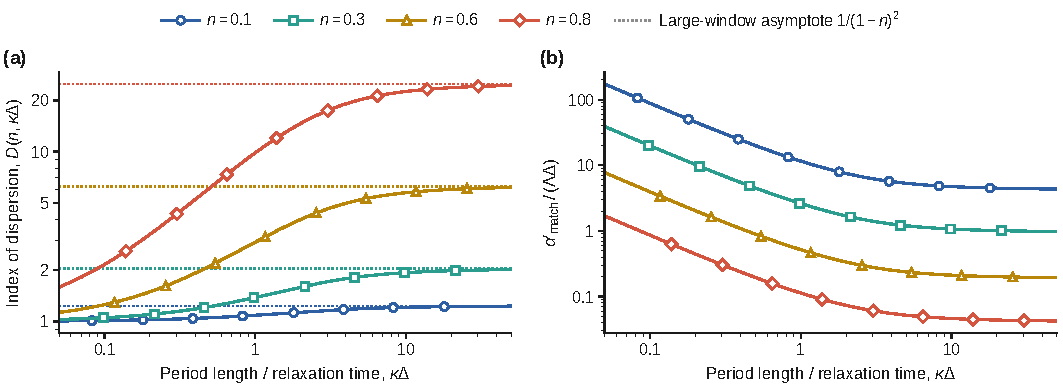
\includegraphics[width=\linewidth]{figs/FigS3_hawkes_dispersion.pdf}
\captionof{figure}{Fig. S3. (a) Index of dispersion (10) of Hawkes window counts against $\kappa\Delta$ for four branching ratios, large-window asymptotes dotted; (b) moment-matched dispersion per unit mean, (11).}\label{fig:S3}\end{minipage}
\vspace{14pt}

\textbf{Supplementary Note 12. Alarm metrics of the robustness arms (Section 5.4 of the main text).}

Table S24 tabulates, for the robustness arms of Section 5.4 that keep the gamma–Poisson truth (the Hawkes arms are in Section 5.4 and Note 11), the M2 alarm metrics that the main text quotes: AUC-PR, Brier score and expected calibration error of the three-month event probability, the one-month detection rates at triage levels 2 and 3, the stable-window false alarms per item-year at level 2, the sequential coverage of the conformal sets, the delay of the $q$ channel after the change, the posterior median of $\alpha'$ and the RMSE of $\log C_i$. Every arm is the reference design ($\alpha' = 2$, $\bar{\mu} = 0.2$, gradual, $I = 30$, $T = 120$) with one factor changed, five replications; the first row is the Study B reference cell (ten replications). Source: \path{results/analysis/R_cells.csv} and \path{B_cells.csv}.

\noindent\begin{minipage}{\linewidth}
\captionof{table}{Table S24. Alarm metrics of M2 in the robustness arms of Section 5.4 (five replications each; the reference cell of Study B, ten replications, for comparison): AUC-PR, Brier score and ECE of the three-month event probability; one-month detection rate at triage levels 2 and 3; stable-window false alarms per item-year at level 2; sequential coverage of the conformal sets (target 0.90); mean delay of the $q$ channel after the change (months); posterior median of $\alpha'$ (truth 2) and RMSE of $\log C_i$.}\label{tab:S24}
\centering\scriptsize
\begin{tabular}{>{\raggedright\arraybackslash}p{2.9cm}rrrrrrrrrrr}
\toprule
Arm & n & AUC-PR & Brier & ECE & DR $\le$ 1 m, L2 & DR $\le$ 1 m, L3 & FA (stable), L2 & Set cov. & $q$ ARL$_1$ & $\alpha'$ median & RMSE $\log C$ \\ \midrule
reference cell (Study B) & 10 & 0.810 & 0.201 & 0.041 & 0.98 & 0.71 & 0.39 & 0.909 & 25.5 & – & – \\
measurement error in $\mathbf{z}$ ($\varsigma$ = 0.5) & 5 & 0.803 & 0.203 & 0.042 & 0.98 & 0.70 & 0.34 & 0.907 & 25.9 & 2.15 & 0.14 \\
15\% missing indicators, latent AR(1) & 5 & 0.825 & 0.193 & 0.041 & 0.98 & 0.73 & 0.45 & 0.914 & 30.5 & 2.12 & 0.14 \\
15\% missing indicators, last value carried forward & 5 & 0.825 & 0.192 & 0.041 & 0.98 & 0.73 & 0.45 & 0.914 & 28.9 & 2.01 & 0.15 \\
Pareto severity & 5 & 0.814 & 0.197 & 0.031 & 0.98 & 0.57 & 0.34 & 0.914 & 27.1 & 1.97 & 0.13 \\
20\% cold-start items & 5 & 0.825 & 0.195 & 0.045 & 0.98 & 0.74 & 0.41 & 0.911 & 24.6 & 2.09 & 0.16 \\
indicator lag 2 in the truth, 1 in the model & 5 & 0.802 & 0.201 & 0.030 & 0.98 & 0.72 & 0.42 & 0.909 & 28.7 & 1.62 & 0.15 \\
\bottomrule
\end{tabular}
\end{minipage}
\vspace{14pt}

\textbf{Supplementary Note 13. Modelling choices and the details of the parameter-recovery results (Sections 3.3 and 5.2 of the main text).}

\textit{Three choices in the intensity dynamics (7)–(9).} First, there is no additional item-period noise term in (7): a log-normal disturbance on $\log R$ and the gamma multiplier in (2) both represent unexplained intensity variation and are not separately identified at small $\mu$ (Table S16 measures the price of fitting the gamma form to a log-normal truth). Second, the level and slope are indexed by group, not item: the item-specific level and the exposure $u_i$ in (14) are identified only through their sum, and item-level slopes cannot be estimated from rare counts (Section 3.2); static item differences therefore live in $C_i$ and the trend in the group, which also lets a cold-start item inherit its group's trajectory. Third, $\sigma_\eta = \tau_\zeta = 0$ reduces (8)–(9) to the deterministic log-linear trend (Y3), so the dynamic model nests the source model (Section 4.1).

\textit{Reference cell: two decisions fed back into the design.} In the single replication of the reference cell reported in Section 5.2, the deterioration probability $P(\delta_t^g > 0.01 \mid \mathcal{D})$ needs a floor: without it the probability floats around one half, with it it averages 0.23 before $t_0$ and 0.76 after $t_0 + 12$. Even the smoothed posterior detects a $+0.02$ per month slope change only seven to eight months after onset, so the slope is a secondary flag and the primary statistics are the level-based $p$ and $q$; and sparse (horseshoe) innovations buy nothing in a gradual regime, so the Gaussian model is the base.

\textit{(i) Pooling.} Complete pooling attributes the residual item heterogeneity to dispersion: coverage of $\log C_i$ falls to 0.13–0.49, and as the information grows its $\alpha'$ intervals contract around a value that is too small—at $\bar{\mu} = 0.5$ and $I = 30$ they cover the truth in 20\% of cases (Fig.~4 of the main text; Table S5). The bias is predictable: an omitted item effect $u_i \sim N(0, \tau_C^2)$ multiplies the gamma variable in (2), and the pseudo-true dispersion of the misspecified model is 1.61 at $\tau_C = 0.3$ and 1.00 at $\tau_C = 0.6$ for the item means of the reference cell (Supplementary Note 3; Table S7). No pooling keeps nominal coverage but learns little about the item-level $\alpha'_i$, whose log-scale interval width stays between 1.7 and 3.2.

\textit{(ii) Dispersion information.} The width of the 90\% interval for $\log\alpha'$ falls by a factor of 2.4–4.9 from $\bar{\mu} = 0.05$ to $\bar{\mu} = 0.5$ at $I = 30$ and by 1.6–3.9 at $I = 10$ (Fig.~4b)—more slowly than the $8/\mu^2$ scaling of Section 3.2 implies, because at small $\bar{\mu}$ the hierarchical prior supplies the information that the counts lack; doubling $T$ narrows it by a further 14–42\%. When the dispersion differs across groups—$\alpha'_g$ = (1, 2, 4) and (0.5, 2, 8)—the hierarchy orders the groups correctly in every replication and covers each group's truth in 93\% and 67\% of cases, whereas complete pooling settles at 1.62 and 1.09 and covers them in 20\% and 0\% (Table S13).

\textit{(iii) Abrupt changes.} With strong data ($I = 30$, $\bar{\mu} \geq 0.2$) the horseshoe variant locates the change sharply—posterior probability 0.65–0.90 on the true month, against 0.06–0.10 with Gaussian innovations—but its fits fail a convergence check in 18 of these 20 replications because the posterior is multimodal in the month of the jump; with weak data it spreads the change over neighbouring months. With either innovation model the 90\% interval for the change date contains the true month in every replication (Table S11).

\textbf{Supplementary Note 14. The backtest on public trade data (Section 5.5 of the main text).}

\textit{Data.} Monthly imports of the Republic of Korea (UN Comtrade reporter 410) by partner at the six-digit HS level, extracted from the UN Comtrade data API on 26 October 2026 with \path{backtest/pull_comtrade_multi.py} for the 65 items of Table S25.2 (five groups: semiconductor chemicals, gases and wafers; battery materials; refractory and minor metals; ferroalloys; rare earths and magnets), 2013-01 to 2025-12 (Korea's monthly series on Comtrade begin in 2013; HS 810291, unwrought molybdenum, is coded 810294 from HS 2007 and returned no records, leaving 64 items). Quantities are net weights in kilograms; the 11\% of partner-month records reported without a weight enter the panel as zero quantity and their value enters the unit value---all 5,440 records of 2013 are among them, so quantities begin in 2014-01, the panel in 2014-02 and complete trailing-twelve-month windows in 2015-01, two years before the first decision month. Export-restriction measures come from three sources merged by \path{backtest/events_restrictions.py}: the OECD Inventory of Export Restrictions on Industrial Raw Materials (complete data set, 2009--2021 at the six-digit level of HS 2007, from the OECD web archive of 12 December 2022, the current location of the file), the Global Trade Alert database (the curated data set `Import and Export Restrictions: Critical Minerals' and a query on the 65 item codes, 1,593 interventions, 2008--2026, extracted through the GTA Data Center on 26 October 2026, CC BY-NC 4.0) and a seed list of eleven documented measures whose announcement and implementation dates were checked against the GTA records (nine matched on partner, implementation month and HS scope; the October 2025 extension of China's rare-earth controls carries the GTA implementation date of 10 November 2026 after its suspension; Zimbabwe's 2022 lithium-ore ban covers no listed item). From the GTA records we keep the five export-type intervention types (export ban, export licensing requirement, export quota, export tax, other export-related non-tariff measure), measures whose affected jurisdictions include the Republic of Korea (which removes measures aimed at other destinations, such as entity-list controls and sanctions packages), measures listing at most 100 HS6 codes (which removes economy-wide frameworks: full export-tariff schedules, catch-all rules, the ratification of an export-control law) and measures whose title does not name sanctions, entity lists or catch-all controls; from the OECD inventory we keep every introduction, increase, extension or revision of a measure (eliminations, decreases and the annual `left unchanged' records are dropped) grouped by country, type, date of introduction and legal basis. A measure recorded by more than one source counts once per partner and month. The resulting table holds 307 measures by 74 implementing jurisdictions, an EU measure counted once per member state (Table S27 lists those that became events).

\textit{An item whose code changed.} Bismuth (HS 810600) has no record under this code after 2021-12. The reason is the 2022 edition of the Harmonized System, which has been in force since January 2022 and divides heading 81.06 into subheadings 8106.10 and 8106.90. Because the records were extracted in the classification as reported, code 810600 does not occur in them from January 2022. As a result, the panel shows zero imports of bismuth in every month of 2022 and has no row for it from 2023-01. It therefore has a row for 6,812 of the 6,848 item-months of the evaluation grid (64 items $\times$ 107 decision months; Table S25.1). Bismuth has 21 trade interruptions (E1 item-months) in the decision window. Of these, 7 fall in 2022, and they result from the change of code, not from a change in supply. Bismuth nevertheless stays in every table, because dropping it changes the results little. We checked this by evaluating the archived alarm paths without bismuth, with no model refitted (\path{backtest/drop_item.py}). Without bismuth, the AUC-PR of M2 is 0.611 instead of 0.600 and its calibration error is 0.024 instead of 0.029. Its detection rate within one month at level 2 stays at 0.91, and its alarm months per item-year are 8.1 instead of 8.2. M2 also remains cheaper than both never acting and always acting for $r$ between 3.0 and 21.

\textit{Events and indicators.} The panel runs from 2014-02, the first month with a positive trailing-twelve-month quantity (the windows are complete from 2015-01), to 2025-12, 143 months, and decisions are made from month 36 (2017-02) to the end, 107 months. A trade interruption (E1) is recorded for item $i$ in month $t$ when a partner that supplied at least a quarter of the item's imports over the trailing twelve months ships less than half of its own trailing-twelve-month median; an export-restriction implementation (E2) when a partner with a trailing share of at least 5\% implements a measure whose HS scope covers the item (exact six-digit code or a two- or four-digit parent); announcement months are recorded separately (E2a) for the lead-time analysis and are never a target. E3 is the union. The first version of the backtest plan used a partner-level definition with a lower share threshold (any partner with a trailing share of at least 5\%); on the 64-item panel it fired in about 35\% of all item-months over 2014--2025 and in 37\% of the decision item-months (4.4 per item-year, a three-month prevalence of 58\%), outside the prevalence range of the simulation design (24--55\% over the three-month horizon, Section 5.1) and high enough to keep the level-2 posture in force in eleven of twelve months. The share threshold was therefore raised to 25\% before the main run and fixed; with it E1 occurs in 17.8\% of the decision item-months (2.1 per item-year; three-month prevalence 34\%). Two alternative definitions---the largest partner's shipments halving, and the item's total imports halving---are reported as sensitivity runs in Table S28; items are screened on data coverage only (at least 60 months with positive imports), never on the number of events. The indicators and exposure measurements are those of Section 5.5 of the main text (partner Herfindahl index, top-partner share, twelve-month change in unit value, three-month growth in quantity; top-partner share and unit-value level over the first 36 months as exposure), lagged one month. The protocol is that of Section 5.3: refits at origins 36, 42, \ldots, 138 (18 origins, two chains of 500 warm-up and 600 sampling iterations), particle propagation between refits, thresholds $\pi = (0.048, 0.167, 0.5)$ with 2-of-2 persistence, the $q$ channel calibrated to ARL$_0 \geq 24$ months in 200 bootstrap paths from the posterior at the first origin (threshold 0.95, persistence 4-of-4, implied ARL$_0$ 2 months), and the baselines of Supplementary Note 2 fitted on the same information set (the LSTM and the temporal fusion transformer of Study B are not refitted here; XGBoost, pooled across the items, represents the machine-learning family, and a second variant holds out the twelve labelled months before each origin, recalibrates the model's probabilities on them by isotonic regression and applies the recalibration until the next origin). Chains start near the prior medians (the median of 15 prior draws per site); a fit whose rank-normalised split-$\widehat{R}$ reached 1.05 or whose bulk effective sample size fell below 100 on any stored quantity ($\boldsymbol{\beta}$, $\alpha'$, $\log C$, the group levels and slopes at the origin, $\sigma_\eta$, $\tau_\zeta$) was repeated once with 1,000 warm-up and 1,000 sampling iterations and kept either way (six of the 18 fits of M2 (origins 36, 42, 54, 126, 132, 138) and none of the 18 fits of the Poisson model); the fits in use have $\widehat{R} \leq 1.043$ and effective sample sizes of at least 56 (the repeated fit still below the criterion: M2 at origin 36, where $\sigma_\eta$ has ESS 56) (\path{results/backtest/main/fits/diagnostics.csv}). A posture dated month $t$ is set on the data through month $t-1$; the probability metrics score $p_{it}(3)$ dated $t$ against an event in months $t$ to $t+2$, the window it predicts, and a shock in month $t$ counts as detected within one month when the level dated $t$ is in force (within three months, when it is in force in any of the months $t-2$ to $t$).

\noindent\begin{minipage}{\linewidth}
\captionof{table}{Table S25.1. Composition of the Korean import panel by group: items, decision item-months (2017-02 to 2025-12), trade interruptions (E1), their share of item-months, export-restriction implementations (E2) and announcements (E2a).}\label{tab:S25_1}
\centering\scriptsize
\begin{tabular}{lrrrrrr}
\toprule
Group & Items & Item-months & E1 & E1 share (\%) & E2 & E2a \\ \midrule
Semiconductor chemicals, gases and wafers & 16 & 1712 & 269 & 15.7 & 14 & 15 \\
Battery materials & 14 & 1498 & 172 & 11.5 & 8 & 7 \\
Refractory and minor metals & 20 & 2104 & 487 & 23.1 & 14 & 13 \\
Ferroalloys & 9 & 963 & 192 & 19.9 & 17 & 16 \\
Rare earths and magnets & 5 & 535 & 93 & 17.4 & 11 & 10 \\
\textbf{All groups} & 64 & 6812 & 1213 & 17.8 & 64 & 61 \\
\bottomrule
\end{tabular}
\end{minipage}
\vspace{14pt}

\noindent\begin{minipage}{\linewidth}
\captionof{table}{Table S25.2. The 65 items: HS 2017 six-digit code, description, group, months with positive imports (2014-02 to 2025-12), and E1 and E2 item-months in the decision window.}\label{tab:S25_2}
\centering\tiny
\begin{tabular}{llp{3.2cm}rrrl}
\toprule
HS6 & Item & Group & Months & E1 & E2 & Note \\ \midrule
281111 & Hydrogen fluoride (hydrofluoric acid) & Semiconductor chemicals & 143 & 5 & 2 &  \\
370790 & Chemical preparations for photographic uses, other (incl. ph & Semiconductor chemicals & 143 & 0 & 1 &  \\
381800 & Chemical elements doped for use in electronics (wafers) & Semiconductor chemicals & 131 & 6 & 4 &  \\
280461 & Silicon, >= 99.99\% Si (polysilicon) & Semiconductor chemicals & 131 & 26 & 1 &  \\
280469 & Silicon, other & Semiconductor chemicals & 143 & 1 & 0 &  \\
280429 & Rare gases other than argon (neon, krypton, xenon) & Semiconductor chemicals & 143 & 10 & 0 &  \\
280421 & Argon & Semiconductor chemicals & 80 & 2 & 0 &  \\
284700 & Hydrogen peroxide & Semiconductor chemicals & 143 & 49 & 1 &  \\
281410 & Ammonia, anhydrous & Semiconductor chemicals & 143 & 34 & 0 &  \\
280610 & Hydrogen chloride (hydrochloric acid) & Semiconductor chemicals & 143 & 2 & 0 &  \\
280800 & Nitric acid; sulphonitric acids & Semiconductor chemicals & 143 & 39 & 0 &  \\
280700 & Sulphuric acid; oleum & Semiconductor chemicals & 131 & 48 & 0 &  \\
280920 & Phosphoric acid and polyphosphoric acids & Semiconductor chemicals & 143 & 5 & 0 &  \\
282619 & Fluorides, other (incl. tungsten hexafluoride) & Semiconductor chemicals & 131 & 4 & 2 &  \\
285000 & Hydrides, nitrides, azides, silicides and borides (incl. sil & Semiconductor chemicals & 131 & 17 & 2 &  \\
281290 & Halides and halide oxides of non-metals, other (incl. NF3) & Semiconductor chemicals & 143 & 21 & 1 &  \\
283691 & Lithium carbonates & Battery materials & 143 & 6 & 1 &  \\
282520 & Lithium oxide and hydroxide & Battery materials & 143 & 10 & 1 &  \\
282690 & Complex fluorine salts, other (incl. LiPF6) & Battery materials & 131 & 0 & 0 &  \\
282200 & Cobalt oxides and hydroxides & Battery materials & 131 & 21 & 1 &  \\
810520 & Cobalt mattes and intermediate products; unwrought cobalt; p & Battery materials & 131 & 21 & 1 &  \\
283324 & Nickel sulphates & Battery materials & 143 & 34 & 0 &  \\
750210 & Nickel, unwrought, not alloyed & Battery materials & 143 & 14 & 0 &  \\
750400 & Nickel powders and flakes & Battery materials & 143 & 20 & 0 &  \\
260400 & Nickel ores and concentrates & Battery materials & 131 & 15 & 0 &  \\
250410 & Natural graphite, powder or flakes & Battery materials & 143 & 3 & 1 &  \\
380110 & Artificial graphite & Battery materials & 131 & 0 & 2 &  \\
282010 & Manganese dioxide & Battery materials & 143 & 25 & 0 &  \\
811100 & Manganese; articles thereof; waste and scrap & Battery materials & 143 & 1 & 1 &  \\
850760 & Lithium-ion accumulators & Battery materials & 143 & 2 & 0 &  \\
811292 & Unwrought gallium, germanium, indium, niobium, vanadium (HS2 & Refractory and minor metals & 143 & 17 & 3 &  \\
282560 & Germanium oxides and zirconium dioxide & Refractory and minor metals & 131 & 8 & 1 &  \\
811010 & Antimony, unwrought; powders & Refractory and minor metals & 143 & 50 & 1 &  \\
282580 & Antimony oxides & Refractory and minor metals & 143 & 12 & 2 &  \\
810194 & Tungsten, unwrought & Refractory and minor metals & 143 & 19 & 1 &  \\
284180 & Tungstates & Refractory and minor metals & 143 & 49 & 1 &  \\
261100 & Tungsten ores and concentrates & Refractory and minor metals & 116 & 23 & 1 &  \\
810320 & Tantalum, unwrought; powders & Refractory and minor metals & 140 & 24 & 0 &  \\
261590 & Niobium, tantalum or vanadium ores and concentrates & Refractory and minor metals & 90 & 9 & 1 &  \\
810291 & Molybdenum, unwrought; powders & Refractory and minor metals & -- & -- & -- & dropped: no data \\
282570 & Molybdenum oxides and hydroxides & Refractory and minor metals & 143 & 39 & 0 &  \\
261310 & Molybdenum ores and concentrates, roasted & Refractory and minor metals & 143 & 5 & 0 &  \\
282530 & Vanadium oxides and hydroxides & Refractory and minor metals & 143 & 31 & 0 &  \\
810411 & Magnesium, unwrought, >= 99.8\% & Refractory and minor metals & 143 & 1 & 1 &  \\
810419 & Magnesium, unwrought, other & Refractory and minor metals & 143 & 7 & 0 &  \\
810600 & Bismuth and articles thereof & Refractory and minor metals & 95 & 21 & 0 & no record after 2021-12 \\
280450 & Boron; tellurium & Refractory and minor metals & 143 & 51 & 2 &  \\
280490 & Selenium & Refractory and minor metals & 143 & 34 & 0 &  \\
810820 & Titanium, unwrought; powders & Refractory and minor metals & 143 & 36 & 0 &  \\
282300 & Titanium oxides & Refractory and minor metals & 143 & 15 & 0 &  \\
811221 & Chromium, unwrought; powders & Refractory and minor metals & 143 & 36 & 0 &  \\
720241 & Ferro-chromium, > 4\% carbon & Ferroalloys & 143 & 19 & 0 &  \\
720249 & Ferro-chromium, other & Ferroalloys & 143 & 24 & 5 &  \\
720260 & Ferro-nickel & Ferroalloys & 143 & 41 & 1 &  \\
720280 & Ferro-tungsten and ferro-silico-tungsten & Ferroalloys & 119 & 27 & 2 &  \\
720270 & Ferro-molybdenum & Ferroalloys & 96 & 38 & 2 &  \\
720292 & Ferro-vanadium & Ferroalloys & 143 & 9 & 2 &  \\
720293 & Ferro-niobium & Ferroalloys & 143 & 4 & 0 &  \\
720221 & Ferro-silicon, > 55\% silicon & Ferroalloys & 143 & 17 & 5 &  \\
720230 & Ferro-silico-manganese & Ferroalloys & 143 & 13 & 0 &  \\
280530 & Rare-earth metals, scandium and yttrium & Rare earths and magnets & 131 & 30 & 4 &  \\
284610 & Cerium compounds & Rare earths and magnets & 143 & 34 & 0 &  \\
284690 & Rare-earth compounds, other & Rare earths and magnets & 143 & 24 & 4 &  \\
850511 & Permanent magnets of metal (incl. NdFeB) & Rare earths and magnets & 131 & 3 & 3 &  \\
850519 & Permanent magnets, other & Rare earths and magnets & 131 & 2 & 0 &  \\
\bottomrule
\end{tabular}
\end{minipage}
\vspace{14pt}

\noindent\begin{minipage}{\linewidth}
\captionof{table}{Table S26.1. Alarm performance on the Korean import panel, target E1: trade interruptions: event probabilities for `at least one event within three months' and the alarm at each level---events flagged within one and within three months before they occur, false alarm onsets per item-year (onsets not followed by an event within three months), alarm months per item-year and lead time in months, median (quartiles); the $q$ channel and the headline level of the two models.}\label{tab:S26_1}
\centering\tiny
\begin{tabular}{lrrrrrrrl}
\toprule
Method & AUC-PR & Brier & ECE & Det.\ $\leq$1 m & Det.\ $\leq$3 m & False alarms & Alarm months & Lead \\ \midrule
M2 (proposed), level 1 & -- & -- & -- & 0.98 & 0.99 & 0.18 & 11.3 & 12.0 (4.0--38.0) \\
M2 (proposed), level 2 & 0.600 & 0.184 & 0.029 & 0.91 & 0.93 & 0.20 & 8.2 & 8.0 (3.0--18.0) \\
M2 (proposed), level 3 & -- & -- & -- & 0.54 & 0.60 & 0.13 & 3.4 & 3.0 (1.0--6.0) \\
M2 (proposed), $q$ channel & -- & -- & -- & 0.00 & 0.00 & -- & 0.0 & -- \\
M2 (proposed), headline (max of level 2 and $q$) & -- & -- & -- & 0.91 & -- & 0.20 & 8.2 & -- \\
Poisson M0, level 1 & -- & -- & -- & 0.99 & 1.00 & 0.12 & 11.7 & 12.0 (3.0--39.0) \\
Poisson M0, level 2 & 0.603 & 0.187 & 0.064 & 0.93 & 0.94 & 0.12 & 8.6 & 6.0 (2.5--13.0) \\
Poisson M0, level 3 & -- & -- & -- & 0.64 & 0.68 & 0.10 & 4.3 & 3.0 (2.0--6.5) \\
Poisson M0, $q$ channel & -- & -- & -- & 0.00 & 0.00 & -- & 0.0 & -- \\
Poisson M0, headline (max of level 2 and $q$) & -- & -- & -- & 0.93 & -- & 0.12 & 8.6 & -- \\
XGBoost (pooled), level 1 & -- & -- & -- & 0.98 & 1.00 & 0.22 & 10.5 & 11.0 (4.0--34.0) \\
XGBoost (pooled), level 2 & 0.661 & 0.167 & 0.022 & 0.88 & 0.91 & 0.25 & 6.8 & 6.0 (2.0--14.0) \\
XGBoost (pooled), level 3 & -- & -- & -- & 0.57 & 0.66 & 0.15 & 3.1 & 2.0 (1.0--5.0) \\
XGBoost, recalibrated, level 1 & -- & -- & -- & 0.98 & 0.99 & 0.25 & 10.3 & 11.0 (3.0--33.0) \\
XGBoost, recalibrated, level 2 & 0.641 & 0.172 & 0.027 & 0.87 & 0.91 & 0.26 & 7.0 & 6.0 (2.0--16.0) \\
XGBoost, recalibrated, level 3 & -- & -- & -- & 0.55 & 0.65 & 0.16 & 3.1 & 2.0 (1.0--5.0) \\
Sigma-rule (plug-in SRI), level 1 & -- & -- & -- & 0.42 & 0.47 & 0.14 & 3.3 & 2.0 (1.0--6.0) \\
Sigma-rule (plug-in SRI), level 2 & -- & -- & -- & 0.30 & 0.35 & 0.14 & 2.0 & 2.0 (1.0--6.2) \\
Sigma-rule (plug-in SRI), level 3 & -- & -- & -- & 0.19 & 0.24 & 0.13 & 1.2 & 2.0 (1.0--5.0) \\
EWMA & -- & -- & -- & 0.24 & 0.29 & 0.11 & 1.4 & 2.0 (1.0--5.0) \\
CUSUM & -- & -- & -- & 0.18 & 0.19 & 0.02 & 1.4 & 1.0 (1.0--4.0) \\
Farrington-type threshold & -- & -- & -- & 0.03 & 0.06 & 0.07 & 0.2 & 2.0 (1.0--12.0) \\
\bottomrule
\end{tabular}
\end{minipage}
\vspace{14pt}

\noindent\begin{minipage}{\linewidth}
\captionof{table}{Table S26.2. Alarm performance on the Korean import panel, target E2: export-restriction implementations: event probabilities for `at least one event within three months' and the alarm at each level---events flagged within one and within three months before they occur, false alarm onsets per item-year (onsets not followed by an event within three months), alarm months per item-year and lead time in months, median (quartiles); the $q$ channel and the headline level of the two models.}\label{tab:S26_2}
\centering\tiny
\begin{tabular}{lrrrrrrrl}
\toprule
Method & AUC-PR & Brier & ECE & Det.\ $\leq$1 m & Det.\ $\leq$3 m & False alarms & Alarm months & Lead \\ \midrule
M2 (proposed), level 1 & -- & -- & -- & 0.91 & 0.91 & 0.22 & 11.3 & 58.0 (14.5--80.0) \\
M2 (proposed), level 2 & 0.025 & 0.205 & 0.341 & 0.61 & 0.66 & 0.26 & 8.2 & 52.0 (15.2--78.0) \\
M2 (proposed), level 3 & -- & -- & -- & 0.22 & 0.30 & 0.32 & 3.4 & 31.0 (10.5--59.0) \\
M2 (proposed), $q$ channel & -- & -- & -- & 0.00 & 0.00 & -- & 0.0 & -- \\
M2 (proposed), headline (max of level 2 and $q$) & -- & -- & -- & 0.61 & -- & 0.26 & 8.2 & -- \\
Poisson M0, level 1 & -- & -- & -- & 0.94 & 0.94 & 0.15 & 11.7 & 61.0 (14.5--91.0) \\
Poisson M0, level 2 & 0.029 & 0.235 & 0.378 & 0.69 & 0.69 & 0.17 & 8.6 & 58.0 (12.8--91.0) \\
Poisson M0, level 3 & -- & -- & -- & 0.33 & 0.36 & 0.19 & 4.3 & 53.0 (11.0--84.8) \\
Poisson M0, $q$ channel & -- & -- & -- & 0.00 & 0.00 & -- & 0.0 & -- \\
Poisson M0, headline (max of level 2 and $q$) & -- & -- & -- & 0.69 & -- & 0.17 & 8.6 & -- \\
XGBoost (pooled), level 1 & -- & -- & -- & 0.92 & 0.95 & 0.26 & 10.5 & 43.0 (11.0--78.0) \\
XGBoost (pooled), level 2 & 0.028 & 0.196 & 0.314 & 0.48 & 0.61 & 0.36 & 6.8 & 40.5 (11.5--77.8) \\
XGBoost (pooled), level 3 & -- & -- & -- & 0.23 & 0.30 & 0.41 & 3.1 & 33.5 (11.0--58.0) \\
XGBoost, recalibrated, level 1 & -- & -- & -- & 0.92 & 0.95 & 0.31 & 10.3 & 59.0 (13.0--78.0) \\
XGBoost, recalibrated, level 2 & 0.026 & 0.196 & 0.319 & 0.48 & 0.62 & 0.39 & 7.0 & 36.0 (12.0--69.0) \\
XGBoost, recalibrated, level 3 & -- & -- & -- & 0.25 & 0.31 & 0.46 & 3.1 & 34.0 (11.0--58.0) \\
Sigma-rule (plug-in SRI), level 1 & -- & -- & -- & 0.20 & 0.30 & 0.34 & 3.3 & 34.0 (14.0--69.5) \\
Sigma-rule (plug-in SRI), level 2 & -- & -- & -- & 0.16 & 0.22 & 0.33 & 2.0 & 35.5 (13.5--61.8) \\
Sigma-rule (plug-in SRI), level 3 & -- & -- & -- & 0.09 & 0.12 & 0.29 & 1.2 & 27.0 (11.5--58.5) \\
EWMA & -- & -- & -- & 0.11 & 0.14 & 0.29 & 1.4 & 31.5 (11.0--57.5) \\
CUSUM & -- & -- & -- & 0.12 & 0.12 & 0.07 & 1.4 & 29.0 (21.0--36.8) \\
Farrington-type threshold & -- & -- & -- & 0.00 & 0.03 & 0.15 & 0.2 & 33.0 (13.0--59.0) \\
\bottomrule
\end{tabular}
\end{minipage}
\vspace{14pt}

\noindent\begin{minipage}{\linewidth}
\captionof{table}{Table S26.3. Alarm performance on the Korean import panel, target E3: union: event probabilities for `at least one event within three months' and the alarm at each level---events flagged within one and within three months before they occur, false alarm onsets per item-year (onsets not followed by an event within three months), alarm months per item-year and lead time in months, median (quartiles); the $q$ channel and the headline level of the two models.}\label{tab:S26_3}
\centering\tiny
\begin{tabular}{lrrrrrrrl}
\toprule
Method & AUC-PR & Brier & ECE & Det.\ $\leq$1 m & Det.\ $\leq$3 m & False alarms & Alarm months & Lead \\ \midrule
M2 (proposed), level 1 & -- & -- & -- & 0.98 & 0.99 & 0.18 & 11.3 & 12.0 (4.0--35.0) \\
M2 (proposed), level 2 & 0.602 & 0.192 & 0.036 & 0.90 & 0.92 & 0.19 & 8.2 & 7.0 (2.5--18.0) \\
M2 (proposed), level 3 & -- & -- & -- & 0.52 & 0.59 & 0.13 & 3.4 & 3.0 (1.0--5.0) \\
M2 (proposed), $q$ channel & -- & -- & -- & 0.00 & 0.00 & -- & 0.0 & -- \\
M2 (proposed), headline (max of level 2 and $q$) & -- & -- & -- & 0.90 & -- & 0.19 & 8.2 & -- \\
Poisson M0, level 1 & -- & -- & -- & 0.98 & 0.99 & 0.12 & 11.7 & 12.0 (3.5--36.5) \\
Poisson M0, level 2 & 0.607 & 0.193 & 0.058 & 0.92 & 0.93 & 0.12 & 8.6 & 6.0 (2.8--13.0) \\
Poisson M0, level 3 & -- & -- & -- & 0.63 & 0.66 & 0.09 & 4.3 & 3.0 (2.0--6.0) \\
Poisson M0, $q$ channel & -- & -- & -- & 0.00 & 0.00 & -- & 0.0 & -- \\
Poisson M0, headline (max of level 2 and $q$) & -- & -- & -- & 0.92 & -- & 0.12 & 8.6 & -- \\
XGBoost (pooled), level 1 & -- & -- & -- & 0.98 & 0.99 & 0.21 & 10.5 & 11.0 (4.0--34.0) \\
XGBoost (pooled), level 2 & 0.662 & 0.176 & 0.035 & 0.86 & 0.89 & 0.25 & 6.8 & 6.0 (2.0--13.0) \\
XGBoost (pooled), level 3 & -- & -- & -- & 0.55 & 0.64 & 0.15 & 3.1 & 2.0 (1.0--4.0) \\
XGBoost, recalibrated, level 1 & -- & -- & -- & 0.97 & 0.99 & 0.25 & 10.3 & 11.0 (3.0--32.0) \\
XGBoost, recalibrated, level 2 & 0.643 & 0.181 & 0.034 & 0.85 & 0.89 & 0.26 & 7.0 & 6.0 (2.0--14.0) \\
XGBoost, recalibrated, level 3 & -- & -- & -- & 0.54 & 0.64 & 0.16 & 3.1 & 2.0 (1.0--4.0) \\
Sigma-rule (plug-in SRI), level 1 & -- & -- & -- & 0.41 & 0.47 & 0.14 & 3.3 & 2.0 (1.0--6.0) \\
Sigma-rule (plug-in SRI), level 2 & -- & -- & -- & 0.29 & 0.34 & 0.14 & 2.0 & 2.0 (1.0--7.0) \\
Sigma-rule (plug-in SRI), level 3 & -- & -- & -- & 0.19 & 0.23 & 0.13 & 1.2 & 2.0 (1.0--5.8) \\
EWMA & -- & -- & -- & 0.23 & 0.28 & 0.11 & 1.4 & 2.0 (1.0--5.0) \\
CUSUM & -- & -- & -- & 0.18 & 0.19 & 0.02 & 1.4 & 1.0 (1.0--4.0) \\
Farrington-type threshold & -- & -- & -- & 0.03 & 0.06 & 0.07 & 0.2 & 3.0 (1.0--12.0) \\
\bottomrule
\end{tabular}
\end{minipage}
\vspace{14pt}

\noindent\begin{minipage}{\linewidth}
\captionof{table}{Table S27. The export-restriction implementations (E2) in the decision window, one row per item and implementation month (a month in which two measures fall on one item is one row): implementation month, item, implementing partner (Comtrade code), measure, and the posture in force in the implementation month, set on the data through the month before (the convention of the detection rates at one month)---the triage level, three-month probability and $q$-alarm of M2 and the months since the item first reached the alert level, the triage level of XGBoost and of the sigma-rule, and the EWMA, CUSUM and Farrington-type alarms. Several items under one measure are separate rows.}\label{tab:S27}
\centering\tiny
\begin{tabular}{lllp{4.2cm}rrrrrrrrr}
\toprule
Month & HS6 & Partner & Measure & M2 lvl & $p(3)$ & $q$ & Since alert & XGB lvl & Sigma lvl & EWMA & CUSUM & Farr. \\ \midrule
2017-06 & 261100 & 643 & Export tax (Resolution of the Government & 2 & 0.42 & no & 3 & 2 & 1 & no & no & no \\
2018-01 & 261590 & 108 & Fiscal tax on exports (Loi No.1/28 du 31 & 1 & 0.09 & no & 10 & 2 & 0 & no & no & no \\
2018-01 & 720221 & 156 & China: 2018 Tariff Implementation Plan r & 2 & 0.20 & no & 10 & 1 & 0 & no & no & no \\
2018-01 & 720249 & 156 & China: 2018 list of licensed ferroalloy  & 3 & 0.56 & no & 10 & 3 & 2 & no & no & no \\
2018-01 & 720270 & 156 & China: 2018 list of licensed ferroalloy  & 2 & 0.33 & no & 10 & 3 & 0 & no & no & no \\
2018-01 & 720280 & 156 & China: 2018 list of licensed ferroalloy  & 3 & 0.66 & no & 10 & 3 & 2 & no & no & no \\
2018-01 & 720292 & 156 & China: 2018 list of licensed ferroalloy  & 2 & 0.47 & no & 10 & 2 & 0 & no & no & no \\
2018-03 & 282200 & 180 & Other export measures (Loi n°18/001 du 0 & 1 & 0.07 & no & 12 & 1 & 0 & no & no & no \\
2018-09 & 283691 & 32 & Export tax (Decreto 793/2018) & 0 & 0.05 & no & -- & 0 & 0 & no & no & no \\
2019-01 & 281111 & 156 & China: 2019 catalogue of 'dual-use' good & 1 & 0.07 & no & -- & 1 & 0 & no & no & no \\
2019-01 & 720221 & 156 & China: 2019 list of licensed ferroalloy  & 2 & 0.27 & no & 22 & 3 & 1 & yes & no & no \\
2019-01 & 720249 & 156 & China: 2019 list of licensed ferroalloy  & 2 & 0.29 & no & 22 & 1 & 0 & no & no & no \\
2019-01 & 720270 & 156 & China: 2019 list of licensed ferroalloy  & 3 & 0.92 & no & 22 & 3 & 2 & no & no & no \\
2019-01 & 720280 & 156 & China: 2019 list of licensed ferroalloy  & 2 & 0.53 & no & 22 & 1 & 0 & no & no & no \\
2019-01 & 720292 & 156 & China: 2019 list of licensed ferroalloy  & 2 & 0.42 & no & 22 & 2 & 0 & no & no & no \\
2019-07 & 281111 & 392 & Export licensing of HF / photoresists /  & 0 & 0.04 & no & -- & 1 & 0 & no & no & no \\
2019-07 & 370790 & 392 & Export licensing of HF / photoresists /  & 2 & 0.35 & no & 28 & 1 & 0 & no & no & no \\
2021-05 & 720221 & 156 & Export tax & 1 & 0.16 & no & 50 & 2 & 0 & no & no & no \\
2021-05 & 720249 & 156 & China: Import/export tariffs on some ste & 1 & 0.21 & no & 50 & 2 & 0 & no & no & no \\
2021-08 & 720249 & 156 & China: Ministry announces export tariffs & 2 & 0.25 & no & 53 & 2 & 0 & no & no & no \\
2021-11 & 720260 & 360 & Indonesia: Introduced export and import  & 3 & 0.60 & no & 56 & 3 & 0 & no & no & no \\
2022-01 & 280530 & 156 & China: 2022 export licensing goods catal & 2 & 0.24 & no & 58 & 2 & 0 & no & no & no \\
2022-01 & 284690 & 156 & China: 2022 export licensing goods catal & 1 & 0.14 & no & 58 & 1 & 0 & no & no & no \\
2022-01 & 720221 & 156 & China: 2022 Tariff Adjustment Plan relea & 1 & 0.12 & no & 58 & 1 & 0 & no & no & no \\
2022-01 & 720249 & 156 & China: 2022 Tariff Adjustment Plan relea & 1 & 0.14 & no & 58 & 1 & 0 & no & no & no \\
2022-01 & 811292 & 156 & China: 2022 export licensing goods catal & 3 & 0.63 & no & 58 & 1 & 0 & no & no & no \\
2023-06 & 811100 & 360 & Indonesia: Introduced export and import  & 0 & 0.04 & no & -- & 1 & 0 & no & no & no \\
2023-08 & 282560 & 156 & Export controls on gallium and germanium & 2 & 0.25 & no & 77 & 2 & 0 & no & no & no \\
2023-08 & 285000 & 156 & China: Government announces export contr & 2 & 0.49 & no & 77 & 2 & 0 & no & yes & no \\
2023-08 & 381800 & 156 & China: Government announces export contr & 1 & 0.07 & no & -- & 1 & 0 & no & no & no \\
2023-08 & 811292 & 156 & Export controls on gallium and germanium & 2 & 0.49 & no & 77 & 1 & 0 & no & no & no \\
2023-12 & 250410 & 156 & Export controls on graphite items & 0 & 0.04 & no & -- & 1 & 0 & no & no & no \\
2023-12 & 380110 & 156 & Export controls on graphite items & 1 & 0.07 & no & -- & 0 & 0 & no & no & no \\
2023-12 & 850511 & 156 & China: Government releases revised catal & 1 & 0.08 & no & 81 & 1 & 0 & no & no & no \\
2024-09 & 282580 & 156 & Export controls on antimony and superhar & 1 & 0.16 & no & 90 & 1 & 0 & no & no & no \\
2024-09 & 285000 & 156 & China: Government announces export contr;842:Uni & 2 & 0.21 & no & 90 & 1 & 0 & no & yes & no \\
2024-09 & 811010 & 156 & Export controls on antimony and superhar & 3 & 0.81 & no & 90 & 3 & 0 & yes & yes & no \\
2025-01 & 280450 & 156 & China: 2025 dual-use catalogue for expor & 3 & 0.82 & no & 94 & 3 & 1 & no & no & no \\
2025-01 & 282580 & 156 & China: 2025 export licensing goods catal & 2 & 0.20 & no & 94 & 2 & 3 & yes & no & no \\
2025-01 & 282619 & 156 & China: 2025 dual-use catalogue for expor & 1 & 0.12 & no & 16 & 0 & 0 & no & no & no \\
2025-01 & 284700 & 156 & China: 2025 dual-use catalogue for expor & 3 & 0.78 & no & 94 & 3 & 0 & no & no & no \\
2025-01 & 380110 & 156 & China: 2025 dual-use catalogue for expor & 1 & 0.08 & no & -- & 1 & 0 & no & no & no \\
2025-01 & 381800 & 156 & China: 2025 dual-use catalogue for expor & 0 & 0.06 & no & -- & 0 & 0 & no & no & no \\
2025-01 & 720221 & 156 & China: 2025 export licensing goods catal & 2 & 0.39 & no & 94 & 3 & 0 & yes & yes & no \\
2025-01 & 810411 & 156 & China: 2025 dual-use catalogue for expor & 1 & 0.06 & no & 78 & 1 & 0 & no & no & no \\
2025-02 & 280450 & 156 & Export controls on tungsten, tellurium,  & 3 & 0.85 & no & 95 & 3 & 3 & no & no & no \\
2025-02 & 284180 & 156 & Export controls on tungsten, tellurium,  & 3 & 0.78 & no & 95 & 1 & 0 & no & no & no \\
2025-02 & 381800 & 156 & China: Government announces export contr & 0 & 0.04 & no & -- & 0 & 0 & no & no & no \\
2025-02 & 810194 & 156 & Export controls on tungsten, tellurium,  & 2 & 0.27 & no & 92 & 1 & 0 & no & no & no \\
2025-02 & 810520 & 180 & Cobalt export suspension & 3 & 0.58 & no & 95 & 3 & 3 & no & no & no \\
2025-02 & 811292 & 156 & Export controls on tungsten, tellurium,  & 2 & 0.50 & no & 95 & 1 & 0 & no & no & no \\
2025-04 & 280530 & 156 & Export controls on seven rare-earth elem & 3 & 0.82 & no & 97 & 3 & 0 & no & no & no \\
2025-04 & 284690 & 156 & Export controls on seven rare-earth elem & 3 & 0.63 & no & 97 & 3 & 3 & yes & yes & no \\
2025-04 & 850511 & 156 & Export controls on seven rare-earth elem & 1 & 0.12 & no & 97 & 1 & 0 & no & no & no \\
2025-05 & 280461 & 392 & Japan: Government tightens the restricti & 2 & 0.50 & no & 98 & 1 & 0 & no & no & no \\
2025-05 & 281290 & 392 & Japan: Government tightens the restricti & 2 & 0.29 & no & 98 & 1 & 0 & no & yes & no \\
2025-05 & 282619 & 392 & Japan: Government tightens the restricti & 1 & 0.08 & no & 20 & 1 & 0 & no & no & no \\
2025-07 & 282520 & 156 & China: Government revises catalogue cont & 2 & 0.28 & no & 74 & 2 & 3 & yes & no & no \\
2025-10 & 280530 & 156 & China: Government announces export contr & 3 & 0.59 & no & 103 & 2 & 0 & no & no & no \\
2025-10 & 284690 & 156 & China: Government announces export contr & 2 & 0.37 & no & 103 & 2 & 0 & no & yes & no \\
2025-10 & 381800 & 156 & China: Ministry of Commerce issues expor & 1 & 0.09 & no & -- & 3 & 3 & yes & no & no \\
2025-11 & 280530 & 156 & Expanded rare-earth export controls (Oct & 2 & 0.49 & no & 104 & 2 & 0 & no & no & no \\
2025-11 & 284690 & 156 & Expanded rare-earth export controls (Oct & 2 & 0.35 & no & 104 & 2 & 0 & no & yes & no \\
2025-11 & 850511 & 156 & Expanded rare-earth export controls (Oct & 1 & 0.07 & no & 104 & 1 & 2 & no & no & no \\
\bottomrule
\end{tabular}
\end{minipage}
\vspace{14pt}

\noindent\begin{minipage}{\linewidth}
\captionof{table}{Table S28. Sensitivity of the backtest to the event definitions, level 2 of the probability-based methods and the sigma-rule: the strict E2 list (new export controls only, annual catalogue and quota renewals excluded; evaluated with the fits of the main run) and the two alternative E1 definitions (the largest partner's shipments halving; the item's total imports halving), each a separate run on the same 64 items. AUC-PR and ECE refer to the E1 probabilities and are not reported for the E2 rows. Last column: event item-months in the decision window.}\label{tab:S28}
\centering\tiny
\begin{tabular}{llrrrrrrr}
\toprule
Variant & Method & AUC-PR & ECE & Det.\ $\leq$1 m & Det.\ $\leq$3 m & False alarms & Alarm months & Events \\ \midrule
E2 strict (new controls only), main fits & M2 (proposed) & -- & -- & 0.65 & 0.65 & 0.26 & 8.2 & 31 \\
E2 strict (new controls only), main fits & Poisson M0 & -- & -- & 0.65 & 0.65 & 0.17 & 8.6 & 31 \\
E2 strict (new controls only), main fits & XGBoost (pooled) & -- & -- & 0.42 & 0.55 & 0.36 & 6.8 & 31 \\
E2 strict (new controls only), main fits & XGBoost, recalibrated & -- & -- & 0.42 & 0.58 & 0.40 & 7.0 & 31 \\
E2 strict (new controls only), main fits & Sigma-rule (plug-in SRI) & -- & -- & 0.16 & 0.23 & 0.33 & 2.0 & 31 \\
E2 strict (new controls only), main fits & EWMA & -- & -- & 0.10 & 0.13 & 0.30 & 1.4 & 31 \\
E2 strict (new controls only), main fits & CUSUM & -- & -- & 0.23 & 0.23 & 0.07 & 1.4 & 31 \\
E2 strict (new controls only), main fits & Farrington-type threshold & -- & -- & 0.00 & 0.03 & 0.15 & 0.2 & 31 \\
E1 = largest partner halves & M2 (proposed) & 0.510 & 0.033 & 0.86 & 0.89 & 0.17 & 7.0 & 926 \\
E1 = largest partner halves & Poisson M0 & 0.517 & 0.040 & 0.88 & 0.90 & 0.11 & 7.5 & 926 \\
E1 = largest partner halves & XGBoost (pooled) & 0.569 & 0.024 & 0.83 & 0.87 & 0.24 & 6.2 & 926 \\
E1 = largest partner halves & XGBoost, recalibrated & 0.555 & 0.025 & 0.81 & 0.87 & 0.30 & 6.2 & 926 \\
E1 = largest partner halves & Sigma-rule (plug-in SRI) & -- & -- & 0.27 & 0.32 & 0.16 & 1.8 & 926 \\
E1 = largest partner halves & EWMA & -- & -- & 0.21 & 0.26 & 0.13 & 1.2 & 926 \\
E1 = largest partner halves & CUSUM & -- & -- & 0.08 & 0.09 & 0.02 & 0.7 & 926 \\
E1 = largest partner halves & Farrington-type threshold & -- & -- & 0.02 & 0.05 & 0.08 & 0.2 & 926 \\
E1 = total imports halve & M2 (proposed) & 0.573 & 0.016 & 0.83 & 0.86 & 0.16 & 5.1 & 750 \\
E1 = total imports halve & Poisson M0 & 0.585 & 0.016 & 0.85 & 0.86 & 0.11 & 5.4 & 750 \\
E1 = total imports halve & XGBoost (pooled) & 0.587 & 0.025 & 0.77 & 0.82 & 0.26 & 4.1 & 750 \\
E1 = total imports halve & XGBoost, recalibrated & 0.570 & 0.020 & 0.77 & 0.84 & 0.33 & 4.4 & 750 \\
E1 = total imports halve & Sigma-rule (plug-in SRI) & -- & -- & 0.26 & 0.32 & 0.16 & 1.7 & 750 \\
E1 = total imports halve & EWMA & -- & -- & 0.23 & 0.29 & 0.14 & 1.2 & 750 \\
E1 = total imports halve & CUSUM & -- & -- & 0.15 & 0.15 & 0.01 & 0.7 & 750 \\
E1 = total imports halve & Farrington-type threshold & -- & -- & 0.02 & 0.04 & 0.09 & 0.1 & 750 \\
\bottomrule
\end{tabular}
\end{minipage}
\vspace{14pt}

\textit{Files.} The panel (\path{backtest/panel_410.csv}), the merged measures (\path{backtest/restrictions.csv}), the extracts of the OECD inventory and of the GTA database for the 65 items, the scripts and the result files of the runs (\path{results/backtest/}) are in the repository; the Comtrade records themselves are not redistributed (UN Comtrade terms of use) and are re-extracted by the script, which needs a free API subscription key.


\textbf{Supplementary Note 15. Conformal prediction sets (Sections 4.3 and 5.3 (iv) of the main text).}

For the observable count $N_{i,t+h}$ the framework forms distribution-free prediction sets from the posterior predictive mass function by the adaptive-prediction-sets construction of Romano et al.\ (2020): the candidate counts are ordered by predictive mass, the set is the smallest initial segment whose cumulative mass reaches the calibrated level, and the level is calibrated on the conformity scores of past item-periods. Because exchangeability fails under regime change, the per-item miscoverage level is adjusted online by adaptive conformal inference (Gibbs and Candès, 2021), which raises the level after a miss and lowers it after a cover, so that the realised sequential coverage tracks the 90\% target; most sets are $\{0\}$ or $\{0,1\}$, and the set size is itself informative. Conformalised quantile regression (Romano et al., 2019) does the same for the loss fraction given a shock (Supplementary Note 8, Table S15). In Study B the sets cover 91.8\% of the counts under M2 with 2.03 counts on average and 90.6\% under the Poisson model with 1.68 (Table 6b of the main text); the gain from modelling over-dispersion lies in the calibration of the event probabilities and in run-length control, not in the prediction sets.

\textbf{Supplementary Note 16. Window-count dispersion of an exponential-kernel Hawkes process (Section 3.4 of the main text).}

Let $\lambda(t) = \nu + \sum_{t_{k} < t} a\, e^{-b(t - t_{k})}$ with $n = a/b < 1$, stationary rate $\Lambda = \nu/(1 - n)$ and $\kappa = b - a = b(1 - n)$. Hawkes (1971) gives the complete covariance density of the stationary process as $\Lambda\,\delta(\tau) + c(\tau)$ with
\begin{equation}
c(\tau) = \frac{\Lambda\, a\,(2b - a)}{2\kappa}\, e^{-\kappa|\tau|}, \qquad \tau \neq 0. \tag{S16.1}
\end{equation}
The variance of the count in a window of length $\Delta$ is the double integral of the covariance density over the window,
\begin{equation}
\mathrm{Var}[N(\Delta)] = \Lambda\Delta + 2\int_{0}^{\Delta} (\Delta - \tau)\, c(\tau)\, d\tau. \tag{S16.2}
\end{equation}
Using $\int_{0}^{\Delta} (\Delta - \tau)\, e^{-\kappa\tau}\, d\tau = \Delta/\kappa - (1 - e^{-\kappa\Delta})/\kappa^{2}$,
\begin{equation}
\mathrm{Var}[N(\Delta)] = \Lambda\Delta\left[1 + \frac{a(2b - a)}{\kappa^{2}}\left(1 - \frac{1 - e^{-\kappa\Delta}}{\kappa\Delta}\right)\right], \tag{S16.3}
\end{equation}
and substituting $a = nb$, $\kappa = b(1 - n)$ gives $a(2b - a)/\kappa^{2} = n(2 - n)/(1 - n)^{2}$, which is (10) of the main text. The large-window limit $1/(1 - n)^{2}$ follows from $1 + n(2 - n)/(1 - n)^{2} = 1/(1 - n)^{2}$, and the small-window expansion from $g(y) = y/2 - y^{2}/6 + O(y^{3})$. The expression agrees with the variance formula of Da Fonseca and Zaatour (2014); Supplementary Note 11 verifies (10)--(11) by exact cluster simulation (Table S23, Fig.~S3).

\textbf{Supplementary Note 17. The rare arm (Sections 5.1, 5.3 and 5.6 of the main text).}

\textbf{Design.} Three cells at a base rate of $\bar{\mu} = 0.02$ shocks per item-month (0.24 per item-year), $I = 100$ items, $T = 120$ months, $G = 3$ groups, $\alpha' = 2$, one per regime---stable, gradual ($+2\%$ per month from $t_0 = 60$) and abrupt ($+\log 3$ at $t_0 = 60$)---with five replications each (cells \texttt{B-a2-mu0.02-\{stable,gradual,abrupt\}-I100}, seeds \texttt{seed\_of("B", cell, rep)}). Everything else is the Study B protocol: the \texttt{t4\_min} design constants (four chains, 400 warm-up and 500 sampling iterations, fourteen origins $36, 42, \dots, 114$, 200 bootstrap paths for the $q$ channel, M0 refitted every four origins), the same decision months, thresholds, persistence rules and metrics (conventions on page 1). The realised three-month event prevalence is 8.2\%, 12.4\% and 16.7\% in the stable, gradual and abrupt cells (24--55\% in Study B), and $E$---shock item-months per item-year over the decision months, an item-month with several shocks counting once---is 0.34, 0.53 and 0.74 (1.13 and 3.15 at the two base rates of Study B); the corresponding numbers of shocks per item-year are 0.36, 0.57 and 0.82. The methods run are M2, the Poisson model M0, XGBoost, the sigma-rule, EWMA and CUSUM; the NB pooling variants, the Farrington-type threshold, the negative-binomial CUSUM and the two recurrent networks (LSTM, TFT) were not run in this arm. All 210 origin fits of M2 passed the convergence check (106 after the one refit; maximum $\widehat{R}$ 1.0099); no M0 fit failed. Conformal coverage was 0.93--0.94 (target 0.90) with 1.0--1.2 counts per set. The arm was run on two CPU cores in 2-hour chunks resumed from an origin-level cache; the two replications of an earlier pilot run on a different machine reproduce to every recorded digit, as the fixed seeds imply.

\textbf{Reading.} Table S29.1 gives the Table 6 metrics by cell and pooled; Table S29.2 the expected cost of Section 5.6, computed as in Table 8 and Tables S21.1--S21.2; Tables S29.3 and S29.4 the per-replication values behind the paired statements of the main text. \emph{Probabilities and triage.} The ranking advantage of M2 over the Poisson model is confined to the abrupt cell (AUC-PR $+0.014$, five of five replications; stable and gradual within $0.004$); the calibration advantage holds in every changing-regime replication (ECE 0.012 and 0.019 against 0.017 and 0.027) and is absent in the stable cell (0.011 against 0.010); XGBoost ranks worse in all fifteen replications and rarely crosses the level-2 threshold. \emph{Change channel.} The $q$ channel of M2 reached the 24-month target in all fifteen bootstrap calibrations (thresholds 0.90--0.975, persistence 2, predicted ARL$_0$ 24--37) and the Poisson channel in nine (one of five in the gradual cell, where even the 0.99 threshold with persistence 3--4 predicted 15--25); in the ten changing-regime replications neither channel alarmed in the 24-month pre-change window, and M2 signalled the change sooner in every replication (abrupt 9.5 against 17.8 months, gradual 33.5 against 43.7). In the stable cell both channels alarmed more often over the 82-month window than the bootstrap had predicted: realised ARL$_0$ (group-months per alarm month) 15, 31, 7, 246 and 13 for M2 and 4, 12, 246, 246 and 8 for the Poisson model, below the target in three of five replications each (246 = no alarm). \emph{Cost.} Against Study B the band in which M2 beats both trivial policies moves from $r \approx 2.6$--19 to $3.6$--66 (pooled) and its centre $12/E$ from 5.4 to 22; the largest saving against the better trivial policy is 22--29\% by cell and 27\% over the three cells (Study B: 30\% over its twelve cells, 23--25\% within a base rate; Table S21.1), against 23--26\% for the Poisson model and 15\% for XGBoost, and it exceeds 10\% for $r$ between 12 and 44 (pooled). The cheapest level of M2 switches from 3 to 2 near $r \approx 10$ and from 2 to 1 near $r \approx 26$ (7 and 18 in Study B). At small ratios there is little to save: at $r = 5$ the three probability-based alarms cost within 2.5\% of never acting in every cell. Paired by replication, at the level that is cheapest on average in the cell (the convention of Table S20; Table S29.4), M2 and the Poisson model cost within 2.3\% of each other in the stable and gradual cells at every tabulated ratio, the Poisson model being the cheaper at some; in the abrupt cell M2 is 1.2--5.2\% cheaper at every tabulated ratio, in four or five of the five replications. Against XGBoost, M2 is 6--17\% cheaper at $r = 20$ and 5--9\% at $r = 50$, in every replication of every cell, and 2--7\% dearer at $r = 2$ in the two changing-regime cells, as in Study B, where the learners are cheaper when misses are cheap. The level of a policy is fixed per cell at each $r$, as in Table 8; choosing it replication by replication, which no policy could do in advance, would lower the pooled cost of XGBoost at $r = 20$ from 9.64 to 9.06 and leave that of M2 at 8.04, narrowing the pooled gap from 17\% to 11\%.

\clearpage
\captionof{table}{Table S29.1. Alarm performance in the rare arm ($\bar{\mu} = 0.02$, $I = 100$, $T = 120$, $\alpha' = 2$; five replications per cell), by cell and pooled, evaluated exactly as Table 6 of the main text. (a) Event probabilities for ``at least one shock within three months'' and triage at level 2 ($\pi_2 = 0.167$, two consecutive months): detection in the month before the shock and within three months, false-alarm onsets per item-year in the stable windows, alarm months per item-year, median lead time (mean of the replication quartiles). (b) Change channel and prediction sets: calibrations reaching the 24-month ARL$_0$ target in the 200 bootstrap paths, the bootstrap-predicted ARL$_0$, the realised ARL$_0$ (median and range over replications; 72 and 246 = no alarm in the 24-month pre-change window or the 82-month stable window), ARL$_1$ (mean over replications; range), conformal coverage and set size.}\label{tab:S29.1}
{\scriptsize
\begin{tabular}{llrrrrrrrl}
\toprule
Cell & Method & AUC-PR & Brier & ECE & Det.\ $\le$1 m & Det.\ $\le$3 m & FA / item-yr & Alarm-mo / item-yr & Lead, median (IQR) \\
\midrule
Stable & M2 (proposed) & 0.164 & 0.073 & 0.011 & 0.20 & 0.26 & 0.18 & 0.9 & 9.2 (3.4--18.1) \\
 & Poisson M0 & 0.168 & 0.073 & 0.010 & 0.20 & 0.25 & 0.16 & 0.8 & 8.8 (3.2--17.2) \\
 & XGBoost & 0.138 & 0.074 & 0.010 & 0.07 & 0.10 & 0.09 & 0.3 & 10.6 (4.0--20.9) \\
 & Sigma-rule, level 2 & -- & -- & -- & 0.23 & 0.37 & 0.69 & 1.7 & 12.5 (4.8--25.4) \\
 & EWMA & -- & -- & -- & 0.11 & 0.16 & 0.18 & 0.9 & 10.4 (4.5--20.2) \\
 & CUSUM & -- & -- & -- & 0.03 & 0.03 & 0.01 & 0.2 & 7.2 (4.8--10.7) \\
\addlinespace
Gradual & M2 (proposed) & 0.278 & 0.101 & 0.012 & 0.42 & 0.48 & 0.29 & 2.1 & 7.4 (3.2--15.9) \\
 & Poisson M0 & 0.281 & 0.101 & 0.017 & 0.38 & 0.45 & 0.26 & 1.8 & 7.0 (3.2--15.2) \\
 & XGBoost & 0.223 & 0.107 & 0.045 & 0.10 & 0.14 & 0.09 & 0.4 & 6.9 (3.0--17.9) \\
 & Sigma-rule, level 2 & -- & -- & -- & 0.32 & 0.47 & 0.83 & 2.4 & 10.5 (4.4--22.6) \\
 & EWMA & -- & -- & -- & 0.19 & 0.25 & 0.25 & 1.3 & 8.7 (4.0--18.3) \\
 & CUSUM & -- & -- & -- & 0.06 & 0.06 & 0.01 & 0.2 & 5.6 (3.9--8.1) \\
\addlinespace
Abrupt & M2 (proposed) & 0.340 & 0.128 & 0.019 & 0.63 & 0.69 & 0.38 & 4.0 & 7.4 (3.0--13.8) \\
 & Poisson M0 & 0.326 & 0.130 & 0.027 & 0.57 & 0.63 & 0.36 & 3.7 & 7.1 (3.0--13.8) \\
 & XGBoost & 0.299 & 0.135 & 0.063 & 0.25 & 0.30 & 0.16 & 1.2 & 5.4 (2.6--11.2) \\
 & Sigma-rule, level 2 & -- & -- & -- & 0.29 & 0.45 & 0.75 & 2.4 & 9.2 (3.8--19.6) \\
 & EWMA & -- & -- & -- & 0.25 & 0.33 & 0.31 & 1.8 & 7.1 (3.0--15.3) \\
 & CUSUM & -- & -- & -- & 0.12 & 0.12 & 0.02 & 0.5 & 4.4 (1.9--7.8) \\
\addlinespace
Pooled & M2 (proposed) & 0.261 & 0.101 & 0.014 & 0.42 & 0.48 & 0.28 & 2.3 & 8.0 (3.2--16.0) \\
 & Poisson M0 & 0.258 & 0.101 & 0.018 & 0.39 & 0.44 & 0.26 & 2.1 & 7.6 (3.1--15.4) \\
 & XGBoost & 0.220 & 0.106 & 0.039 & 0.14 & 0.18 & 0.12 & 0.7 & 7.6 (3.2--16.7) \\
 & Sigma-rule, level 2 & -- & -- & -- & 0.28 & 0.43 & 0.76 & 2.2 & 10.7 (4.3--22.6) \\
 & EWMA & -- & -- & -- & 0.18 & 0.25 & 0.25 & 1.3 & 8.7 (3.9--17.9) \\
 & CUSUM & -- & -- & -- & 0.07 & 0.07 & 0.01 & 0.3 & 5.7 (3.5--8.8) \\
\bottomrule
\end{tabular}

\vspace{4pt}
(b) Change channel and prediction sets

\begin{tabular}{llcccccc}
\toprule
Cell & Channel & Calibrated & Predicted ARL$_0$ & Realised ARL$_0$, median (range) & ARL$_1$, mean (range) & Set coverage & Set size \\
\midrule
Stable & $q$ channel, M2 & 5/5 & 25--37 & 15 (7--246) & -- & 0.928 & 1.01 \\
 & $q$ channel, Poisson M0 & 4/5 & 14--29 & 12 (4--246) & -- & -- & -- \\
 & EWMA & -- & 24 (nominal) & 14 (12--17) & -- & -- & -- \\
 & CUSUM & -- & 24 (nominal) & 76 (52--117) & -- & -- & -- \\
\addlinespace
Gradual & $q$ channel, M2 & 5/5 & 27--35 & 72 (72--72) & 33.5 (28--49) & 0.937 & 1.09 \\
 & $q$ channel, Poisson M0 & 1/5 & 15--25 & 72 (72--72) & 43.7 (35--57) & -- & -- \\
 & EWMA & -- & 24 (nominal) & 17 (14--23) & 31.9 (30--35) & -- & -- \\
 & CUSUM & -- & 24 (nominal) & 2400 (2400--2400) & 56.5 (56--57) & -- & -- \\
\addlinespace
Abrupt & $q$ channel, M2 & 5/5 & 24--33 & 72 (72--72) & 9.5 (4--22) & 0.943 & 1.19 \\
 & $q$ channel, Poisson M0 & 4/5 & 13--27 & 72 (72--72) & 17.8 (11--36) & -- & -- \\
 & EWMA & -- & 24 (nominal) & 16 (15--23) & 22.2 (18--27) & -- & -- \\
 & CUSUM & -- & 24 (nominal) & 2400 (2400--2400) & 54.2 (53--55) & -- & -- \\
\addlinespace
Pooled & $q$ channel, M2 & 15/15 & 24--37 & 72 (7--246) & 21.5 (4--49) & 0.936 & 1.10 \\
 & $q$ channel, Poisson M0 & 9/15 & 13--29 & 72 (4--246) & 30.7 (11--57) & -- & -- \\
 & EWMA & -- & 24 (nominal) & 16 (12--23) & 27.1 (18--35) & -- & -- \\
 & CUSUM & -- & 24 (nominal) & 2400 (52--2400) & 55.3 (53--57) & -- & -- \\
\bottomrule
\end{tabular}}

Realised ARL$_0$ of the $q$ channels is in group-months (three groups), of EWMA and CUSUM in item-months (100 items), as in Table 6; the stable window is the 24 decision months before the change in the gradual and abrupt cells (72 group-months, 2,400 item-months) and all 82 decision months in the stable cell (246 and 8,200).

\clearpage
\captionof{table}{Table S29.2. Expected cost per item-year in the rare arm (Model A of Section 5.6, units of one alarm-month), by cell and pooled over the fifteen replications, computed as in Table 8: for each policy the lower envelope of its level-wise mean-cost lines (eq. 21), i.e. the mean over replications at the level that is cheapest on average at that $r$, with the standard error in brackets, at $r$ = 2, 5, 10, 20 and 50. The last three columns give, as in Tables S21.1 and S21.2, the band of $r$ in which the policy is cheaper than the better of never and always acting, $\min(rE, 12)$ with $E$ the mean of the subset, its largest saving against that policy, which lies at $r = 12/E$ (34.9, 22.6, 16.2; 22.3 pooled), and the range of $r$ over which the saving exceeds 10\%. Never act costs $rE$ per item-year ($E$ = 0.34, 0.53, 0.74; 0.54 pooled); always act costs 12.}\label{tab:S29.2}
{\scriptsize
\begin{tabular}{llrrrrrccc}
\toprule
Cell & Method & $r=2$ & $r=5$ & $r=10$ & $r=20$ & $r=50$ & Band of $r$ & Largest saving & Saving $>$ 10\% \\
\midrule
Stable & M2 (proposed) & 0.69 (0.02) & 1.72 (0.05) & 3.44 (0.10) & 6.36 (0.09) & 10.42 (0.16) & 4.1--72 & 22\% & 25--55 \\
 & Poisson M0 & 0.69 (0.02) & 1.72 (0.05) & 3.44 (0.10) & 6.28 (0.09) & 10.39 (0.11) & 4.3--72 & 23\% & 22--56 \\
 & XGBoost & 0.69 (0.02) & 1.72 (0.05) & 3.44 (0.10) & 6.74 (0.16) & 11.23 (0.14) & 14.0--62 & 15\% & 33--43 \\
 & Sigma-rule (3 limits) & 1.72 (0.06) & 2.60 (0.07) & 4.05 (0.11) & 6.96 (0.20) & 13.96 (0.31) & 21.3--41 & 12\% & 31--36 \\
 & EWMA & 1.47 (0.06) & 2.38 (0.07) & 3.90 (0.11) & 6.95 (0.19) & 16.09 (0.43) & 21.7--37 & 4\% & -- \\
 & CUSUM & 0.83 (0.04) & 1.83 (0.06) & 3.49 (0.10) & 6.81 (0.17) & 16.79 (0.40) & 14.1--36 & 2\% & -- \\
 & Never act & 0.69 (0.02) & 1.72 (0.05) & 3.44 (0.10) & 6.88 (0.20) & 17.21 (0.50) & -- & -- & -- \\
 & Always act & 12.00 & 12.00 & 12.00 & 12.00 & 12.00 & -- & -- & -- \\
\addlinespace
Gradual & M2 (proposed) & 1.08 (0.02) & 2.62 (0.06) & 5.16 (0.17) & 8.25 (0.27) & 11.23 (0.12) & 3.3--64 & 24\% & 12--42 \\
 & Poisson M0 & 1.08 (0.02) & 2.62 (0.06) & 5.05 (0.16) & 8.32 (0.24) & 11.26 (0.19) & 3.2--62 & 24\% & 12--43 \\
 & XGBoost & 1.06 (0.02) & 2.65 (0.06) & 5.14 (0.16) & 9.89 (0.38) & 12.36 (0.14) & $<$1--45$^{a}$ & 15\% & 21--31 \\
 & Sigma-rule (3 limits) & 2.44 (0.07) & 3.66 (0.09) & 5.69 (0.13) & 9.40 (0.16) & 18.35 (0.26) & 13.1--29 & 15\% & 19--25 \\
 & EWMA & 2.19 (0.08) & 3.48 (0.11) & 5.63 (0.17) & 9.93 (0.31) & 22.83 (0.76) & 13.3--25 & 8\% & -- \\
 & CUSUM & 1.21 (0.02) & 2.71 (0.06) & 5.21 (0.14) & 10.21 (0.29) & 25.20 (0.73) & 7.1--24 & 4\% & -- \\
 & Never act & 1.06 (0.02) & 2.65 (0.06) & 5.30 (0.12) & 10.60 (0.23) & 26.50 (0.58) & -- & -- & -- \\
 & Always act & 12.00 & 12.00 & 12.00 & 12.00 & 12.00 & -- & -- & -- \\
\addlinespace
Abrupt & M2 (proposed) & 1.59 (0.05) & 3.60 (0.08) & 6.77 (0.09) & 9.51 (0.12) & 11.73 (0.16) & 3.7--57 & 29\% & 10--26 \\
 & Poisson M0 & 1.62 (0.06) & 3.65 (0.08) & 6.87 (0.11) & 10.03 (0.20) & 11.96 (0.22) & 4.3--51 & 26\% & 11--25 \\
 & XGBoost & 1.49 (0.04) & 3.68 (0.08) & 6.77 (0.12) & 10.70 (0.15) & 12.32 (0.17) & 3.3--44 & 15\% & 11--22 \\
 & Sigma-rule (3 limits) & 2.80 (0.06) & 4.55 (0.10) & 7.47 (0.16) & 12.10 (0.18) & 25.16 (0.38) & 10.5--20 & 13\% & 15--17 \\
 & EWMA & 2.92 (0.07) & 4.58 (0.08) & 7.36 (0.10) & 12.92 (0.15) & 29.61 (0.35) & 9.9--18 & 10\% & -- \\
 & CUSUM & 1.83 (0.07) & 3.79 (0.08) & 7.06 (0.11) & 13.58 (0.21) & 33.16 (0.51) & 6.2--18 & 7\% & -- \\
 & Never act & 1.48 (0.03) & 3.69 (0.08) & 7.39 (0.17) & 14.77 (0.33) & 36.94 (0.84) & -- & -- & -- \\
 & Always act & 12.00 & 12.00 & 12.00 & 12.00 & 12.00 & -- & -- & -- \\
\addlinespace
Pooled & M2 (proposed) & 1.12 (0.10) & 2.65 (0.21) & 5.19 (0.35) & 8.04 (0.36) & 11.12 (0.16) & 3.6--66 & 27\% & 12--44 \\
 & Poisson M0 & 1.13 (0.10) & 2.66 (0.21) & 5.16 (0.37) & 8.21 (0.42) & 11.20 (0.20) & 4.0--63 & 26\% & 12--43 \\
 & XGBoost & 1.08 (0.09) & 2.68 (0.22) & 5.15 (0.36) & 9.64 (0.63) & 11.97 (0.16) & 3.6--50 & 16\% & 19--32 \\
 & Sigma-rule (3 limits) & 2.32 (0.12) & 3.60 (0.22) & 5.74 (0.38) & 9.53 (0.55) & 19.16 (1.24) & 13.2--28 & 14\% & 19--24 \\
 & EWMA & 2.19 (0.16) & 3.48 (0.24) & 5.63 (0.38) & 9.94 (0.66) & 22.84 (1.50) & 12.4--25 & 9\% & -- \\
 & CUSUM & 1.29 (0.11) & 2.78 (0.22) & 5.25 (0.39) & 10.20 (0.75) & 25.05 (1.81) & 7.1--24 & 5\% & -- \\
 & Never act & 1.08 (0.09) & 2.69 (0.22) & 5.38 (0.44) & 10.75 (0.87) & 26.88 (2.18) & -- & -- & -- \\
 & Always act & 12.00 & 12.00 & 12.00 & 12.00 & 12.00 & -- & -- & -- \\
\bottomrule
\end{tabular}}

$^{a}$ XGBoost in the gradual cell: the level-3 alarm is almost never in force, so that the policy costs less than never acting from $r = 1$ by under 1\%; its saving exceeds 1\% for $r$ between 8 and 44.

Levels used at $r$ = 2/5/10/20/50 (the cheapest on average): stable: M2 3/3/3/2/1, Poisson M0 3/3/3/2/1, XGBoost 3/3/3/2/1, sigma-rule limit 3/3/3/3/1; gradual: M2 3/3/2/2/1, Poisson M0 3/3/2/2/1, XGBoost 3/3/2/2/1, sigma-rule limit 3/3/3/1/1; abrupt: M2 3/3/2/2/1, Poisson M0 3/3/2/2/1, XGBoost 3/3/2/1/1, sigma-rule limit 3/3/3/1/1; pooled: M2 3/3/2/2/1, Poisson M0 3/3/2/2/1, XGBoost 3/3/2/2/1, sigma-rule limit 3/3/3/1/1.

\vspace{8pt}
\captionof{table}{Table S29.3. The rare arm replication by replication: AUC-PR and ECE of the event probabilities for M2, the Poisson model and XGBoost, the level-2 detection share within one month, and the realised ARL$_0$ and ARL$_1$ of the two $q$ channels (group-months; 72 and 246 = no alarm; ARL$_1$ in months after the change). The paired differences quoted in the main text are computed within these rows: AUC-PR of M2 exceeds that of the Poisson model in 1/5, 2/5 and 5/5 replications of the stable, gradual and abrupt cells and that of XGBoost in 15/15; the ECE of M2 is below that of the Poisson model in 3/5, 5/5 and 5/5 and below that of XGBoost in 2/5, 5/5 and 5/5.}\label{tab:S29.3}
{\scriptsize
\begin{tabular}{lrrrrrrrrrrrrr}
\toprule
 & & \multicolumn{3}{c}{AUC-PR} & \multicolumn{3}{c}{ECE} & \multicolumn{3}{c}{Det.\ $\le$1 m, level 2} & \multicolumn{2}{c}{$q$ channel ARL$_0$ / ARL$_1$} \\
\cmidrule(lr){3-5}\cmidrule(lr){6-8}\cmidrule(lr){9-11}\cmidrule(lr){12-13}
Cell & Rep & M2 & M0 & XGB & M2 & M0 & XGB & M2 & M0 & XGB & M2 & M0 \\
\midrule
Stable & 0 & 0.149 & 0.152 & 0.130 & 0.0131 & 0.0063 & 0.0101 & 0.17 & 0.16 & 0.05 & 15 / -- & 4 / -- \\
 & 1 & 0.141 & 0.139 & 0.121 & 0.0165 & 0.0171 & 0.0046 & 0.16 & 0.14 & 0.06 & 31 / -- & 12 / -- \\
 & 2 & 0.138 & 0.143 & 0.110 & 0.0106 & 0.0063 & 0.0083 & 0.13 & 0.12 & 0.05 & 7 / -- & 246 / -- \\
 & 3 & 0.190 & 0.194 & 0.163 & 0.0050 & 0.0067 & 0.0121 & 0.26 & 0.29 & 0.08 & 246 / -- & 246 / -- \\
 & 4 & 0.202 & 0.209 & 0.163 & 0.0096 & 0.0116 & 0.0157 & 0.28 & 0.31 & 0.10 & 13 / -- & 8 / -- \\
\addlinespace
Gradual & 0 & 0.232 & 0.230 & 0.192 & 0.0172 & 0.0221 & 0.0479 & 0.37 & 0.35 & 0.06 & 72 / 31 & 72 / 35 \\
 & 1 & 0.266 & 0.270 & 0.196 & 0.0208 & 0.0254 & 0.0548 & 0.43 & 0.39 & 0.05 & 72 / 28 & 72 / 38 \\
 & 2 & 0.302 & 0.311 & 0.241 & 0.0072 & 0.0161 & 0.0470 & 0.50 & 0.41 & 0.07 & 72 / 29 & 72 / 47 \\
 & 3 & 0.306 & 0.303 & 0.242 & 0.0093 & 0.0141 & 0.0335 & 0.40 & 0.38 & 0.19 & 72 / 49 & 72 / 57 \\
 & 4 & 0.282 & 0.288 & 0.243 & 0.0075 & 0.0090 & 0.0400 & 0.40 & 0.38 & 0.15 & 72 / 30 & 72 / 41 \\
\addlinespace
Abrupt & 0 & 0.317 & 0.311 & 0.278 & 0.0205 & 0.0231 & 0.0629 & 0.62 & 0.58 & 0.18 & 72 / 10 & 72 / 14 \\
 & 1 & 0.354 & 0.339 & 0.322 & 0.0187 & 0.0315 & 0.0713 & 0.63 & 0.58 & 0.28 & 72 / 5 & 72 / 13 \\
 & 2 & 0.361 & 0.338 & 0.315 & 0.0168 & 0.0200 & 0.0502 & 0.63 & 0.62 & 0.34 & 72 / 22 & 72 / 36 \\
 & 3 & 0.304 & 0.300 & 0.270 & 0.0174 & 0.0287 & 0.0705 & 0.62 & 0.50 & 0.15 & 72 / 6 & 72 / 11 \\
 & 4 & 0.365 & 0.341 & 0.311 & 0.0214 & 0.0330 & 0.0603 & 0.65 & 0.58 & 0.31 & 72 / 4 & 72 / 15 \\
\bottomrule
\end{tabular}}

\clearpage
\captionof{table}{Table S29.4. Expected cost replication by replication in the rare arm (units of one alarm-month per item-year): $E_j$, the shock item-months per item-year of the replication, and the cost (21) of M2, the Poisson model and XGBoost at $r$ = 2, 5, 10, 20 and 50, each at the level that is cheapest on average in its cell at that $r$ (the levels listed under Table S29.2). The paired statements of Section 5.6 are computed within these rows; never acting costs $rE_j$ and always acting 12.}\label{tab:S29.4}
{\scriptsize
\setlength{\tabcolsep}{3pt}
\begin{tabular}{lrr*{5}{rrr}}
\toprule
 & & & \multicolumn{3}{c}{$r=2$} & \multicolumn{3}{c}{$r=5$} & \multicolumn{3}{c}{$r=10$} & \multicolumn{3}{c}{$r=20$} & \multicolumn{3}{c}{$r=50$} \\
\cmidrule(lr){4-6}\cmidrule(lr){7-9}\cmidrule(lr){10-12}\cmidrule(lr){13-15}\cmidrule(lr){16-18}
Cell & Rep & $E_j$ & M2 & M0 & XGB & M2 & M0 & XGB & M2 & M0 & XGB & M2 & M0 & XGB & M2 & M0 & XGB \\
\midrule
Stable & 0 & 0.347 & 0.69 & 0.69 & 0.69 & 1.73 & 1.73 & 1.73 & 3.47 & 3.47 & 3.47 & 6.57 & 6.54 & 6.92 & 10.09 & 10.59 & 11.17 \\
 & 1 & 0.318 & 0.64 & 0.64 & 0.64 & 1.59 & 1.59 & 1.59 & 3.17 & 3.18 & 3.18 & 6.08 & 6.01 & 6.29 & 10.12 & 10.17 & 11.47 \\
 & 2 & 0.325 & 0.65 & 0.65 & 0.65 & 1.62 & 1.62 & 1.63 & 3.25 & 3.25 & 3.25 & 6.25 & 6.19 & 6.44 & 10.75 & 10.47 & 11.50 \\
 & 3 & 0.364 & 0.73 & 0.73 & 0.73 & 1.82 & 1.82 & 1.82 & 3.63 & 3.63 & 3.65 & 6.55 & 6.41 & 7.10 & 10.29 & 10.09 & 10.74 \\
 & 4 & 0.367 & 0.74 & 0.74 & 0.74 & 1.84 & 1.83 & 1.84 & 3.67 & 3.65 & 3.68 & 6.38 & 6.26 & 6.96 & 10.84 & 10.62 & 11.27 \\
 & mean & 0.344 & 0.69 & 0.69 & 0.69 & 1.72 & 1.72 & 1.72 & 3.44 & 3.44 & 3.44 & 6.36 & 6.28 & 6.74 & 10.42 & 10.39 & 11.23 \\
\addlinespace
Gradual & 0 & 0.522 & 1.06 & 1.07 & 1.04 & 2.62 & 2.64 & 2.61 & 5.44 & 5.37 & 5.22 & 8.75 & 8.75 & 10.11 & 11.47 & 11.39 & 12.07 \\
 & 1 & 0.574 & 1.17 & 1.15 & 1.15 & 2.83 & 2.81 & 2.87 & 5.69 & 5.52 & 5.68 & 8.97 & 9.02 & 11.13 & 11.52 & 11.91 & 12.85 \\
 & 2 & 0.528 & 1.11 & 1.09 & 1.06 & 2.63 & 2.63 & 2.64 & 4.95 & 4.74 & 5.14 & 7.61 & 7.84 & 10.06 & 10.90 & 10.91 & 12.50 \\
 & 3 & 0.521 & 1.06 & 1.05 & 1.04 & 2.52 & 2.53 & 2.60 & 4.97 & 4.83 & 4.90 & 8.12 & 8.05 & 9.15 & 11.06 & 10.86 & 12.11 \\
 & 4 & 0.505 & 1.03 & 1.04 & 1.01 & 2.48 & 2.49 & 2.52 & 4.77 & 4.79 & 4.75 & 7.78 & 7.92 & 9.03 & 11.20 & 11.22 & 12.29 \\
 & mean & 0.530 & 1.08 & 1.08 & 1.06 & 2.62 & 2.62 & 2.65 & 5.16 & 5.05 & 5.14 & 8.25 & 8.32 & 9.89 & 11.23 & 11.26 & 12.36 \\
\addlinespace
Abrupt & 0 & 0.723 & 1.51 & 1.53 & 1.45 & 3.53 & 3.55 & 3.61 & 6.96 & 6.95 & 6.94 & 9.72 & 9.99 & 11.27 & 12.26 & 12.32 & 12.41 \\
 & 1 & 0.790 & 1.76 & 1.81 & 1.62 & 3.90 & 3.93 & 3.95 & 6.94 & 7.19 & 7.12 & 9.85 & 10.52 & 10.46 & 11.58 & 12.13 & 12.53 \\
 & 2 & 0.729 & 1.58 & 1.62 & 1.46 & 3.50 & 3.55 & 3.60 & 6.52 & 6.56 & 6.42 & 9.20 & 9.33 & 10.45 & 11.29 & 11.13 & 11.67 \\
 & 3 & 0.692 & 1.45 & 1.46 & 1.39 & 3.45 & 3.47 & 3.46 & 6.62 & 6.72 & 6.64 & 9.29 & 10.19 & 10.76 & 11.72 & 12.23 & 12.65 \\
 & 4 & 0.760 & 1.65 & 1.68 & 1.54 & 3.63 & 3.73 & 3.77 & 6.82 & 6.94 & 6.73 & 9.51 & 10.13 & 10.58 & 11.77 & 12.00 & 12.34 \\
 & mean & 0.739 & 1.59 & 1.62 & 1.49 & 3.60 & 3.65 & 3.68 & 6.77 & 6.87 & 6.77 & 9.51 & 10.03 & 10.70 & 11.73 & 11.96 & 12.32 \\
\bottomrule
\end{tabular}}




\vspace{10pt}

\textbf{References cited in Supplementary Notes 7–11, 15 and 16.} Cameron, A.C., Trivedi, P.K., 2013. Regression Analysis of Count Data, 2nd ed. Cambridge University Press, Cambridge. Coles, S., 2001. An Introduction to Statistical Modeling of Extreme Values. Springer, London. Credit Suisse Financial Products, 1997. CreditRisk+: A Credit Risk Management Framework. London. Cunningham, J.A., 1990. IEEE Trans. Semicond. Manuf. 3, 60–71. Da Fonseca, J., Zaatour, R., 2014. J. Futures Mark. 34, 548–579. Ferrari, S., Cribari-Neto, F., 2004. J. Appl. Stat. 31, 799–815. Gibbs, I., Candès, E., 2021. Adv. Neural Inf. Process. Syst. 34, 1660–1672. Goel, A.L., Okumoto, K., 1979. IEEE Trans. Reliab. R-28, 206–211. Grandell, J., 1997. Mixed Poisson Processes. Chapman \& Hall, London. Greenwood, M., Yule, G.U., 1920. J. R. Stat. Soc. 83, 255–279. Hawkes, A.G., 1971. Biometrika 58, 83–90. Hawkes, A.G., Oakes, D., 1974. J. Appl. Probab. 11, 493–503. Hougaard, P., 2000. Analysis of Multivariate Survival Data. Springer, New York. Lawless, J.F., 1987. Can. J. Stat. 15, 209–225. Lloyd-Smith, J.O., et al., 2005. Nature 438, 355–359. Murphy, B.T., 1964. Proc. IEEE 52, 1537–1545. Ospina, R., Ferrari, S.L.P., 2010. Stat. Pap. 51, 111–126. Pickands, J., 1975. Ann. Stat. 3, 119–131. Price, J.E., 1970. Proc. IEEE 58, 1290–1291. Romano, Y., Patterson, E., Candès, E., 2019. Adv. Neural Inf. Process. Syst. 32, 3538–3548. Romano, Y., Sesia, M., Candès, E., 2020. Adv. Neural Inf. Process. Syst. 33, 3581–3591. Seeds, R.B., 1967. IEEE Int. Conv. Rec. 6, 60–61. Smithson, M., Verkuilen, J., 2006. Psychol. Methods 11, 54–71. Stapper, C.H., 1973. IEEE Trans. Electron Devices 20, 655–657. Stapper, C.H., 1989. Microelectron. J. 20, 129–151. Stapper, C.H., Armstrong, F.M., Saji, K., 1983. Proc. IEEE 71, 453–470. Vaupel, J.W., Manton, K.G., Stallard, E., 1979. Demography 16, 439–454. Wright, T.P., 1936. J. Aeronaut. Sci. 3, 122–128.
